\documentclass[11pt,letterpaper]{article}

% --- PAQUETES DE CONFIGURACIÓN BÁSICA ---
\usepackage[utf8]{inputenc}
\renewcommand{\contentsname}{Índice General de Contenidos}
\renewcommand{\tablename}{Tabla}
\renewcommand{\figurename}{Figura}
\AtBeginDocument{\renewcommand{\contentsname}{Índice General de Contenidos}}
\usepackage[margin=2.0cm,top=2.5cm,bottom=2.5cm]{geometry}
\usepackage{amsmath,amssymb,amsfonts}
\usepackage{graphicx}
\usepackage{booktabs}
\usepackage{tabularx}
\usepackage{xltabular}
\usepackage{array}
\usepackage{colortbl}
\usepackage{pdflscape}
\usepackage{float}
\usepackage{fancyhdr}
\usepackage{lastpage}
\usepackage{tikz}
\usepackage{enumitem}
\usepackage{listings}
\usepackage{xcolor}
\usepackage{tcolorbox}
\tcbuselibrary{skins,breakable}

% --- PALETA DE COLORES SOLVANTA ---
\definecolor{primaryblue}{HTML}{0A2540}
\definecolor{secondaryblue}{HTML}{0070BA}
\definecolor{accentteal}{HTML}{00A3BF}
\definecolor{darkslate}{HTML}{203A43}
\definecolor{lightbg}{HTML}{F8FAFC}
\definecolor{tableheader}{HTML}{0A2540}
\definecolor{tablerowgray}{HTML}{F1F5F9}
\definecolor{alertred}{HTML}{C53030}
\definecolor{alertbg}{HTML}{FFF5F5}
\definecolor{warngold}{HTML}{DD6B20}
\definecolor{warnbg}{HTML}{FFFAF0}
\definecolor{boxborder}{HTML}{CBD5E1}
\definecolor{codebg}{HTML}{1E293B}
\definecolor{codetext}{HTML}{F8FAFC}
\definecolor{codekw}{HTML}{38BDF8}
\definecolor{codestrg}{HTML}{34D399}
\definecolor{codecomment}{HTML}{94A3B8}

% --- CONFIGURACIÓN DE LISTINGS (PYTHON / BIOSTEAM) ---
\lstdefinestyle{biosteamstyle}{
    language=Python,
    backgroundcolor=\color{lightbg},
    basicstyle=\ttfamily\footnotesize\color{darkslate},
    keywordstyle=\color{secondaryblue}\bfseries,
    stringstyle=\color{accentteal},
    commentstyle=\color{codecomment}\itshape,
    numberstyle=\tiny\color{codecomment},
    numbers=left,
    numbersep=6pt,
    stepnumber=1,
    tabsize=4,
    showstringspaces=false,
    breaklines=true,
    breakatwhitespace=false,
    frame=single,
    rulecolor=\color{boxborder},
    xleftmargin=12pt,
    framexleftmargin=8pt,
    morekeywords={self, Unit, Stream, System, TEA, Mixer, Splitter, HXutility, BinaryDistillation, Flash, ins, outs, design_results, baseline_purchase_costs, installed_costs, purchase_cost, installed_equipment_cost, FCI, TCI, VOC, FOC, AOC, solve_price, solve_IRR, get_cashflow_table}
}
\lstset{style=biosteamstyle}

% --- HIPERVÍNCULOS ---
\usepackage[colorlinks=true,
            linkcolor=primaryblue,
            citecolor=accentteal,
            urlcolor=secondaryblue]{hyperref}

% --- ENCABEZADOS Y PIES DE PÁGINA ---
\pagestyle{fancy}
\fancyhf{}
\renewcommand{\headrulewidth}{0.6pt}
\renewcommand{\footrulewidth}{0.4pt}
\fancyhead[L]{\small\bfseries\color{primaryblue}Solvanta Engineering Solutions S.A. de C.V.}
\fancyhead[R]{\small\color{darkslate}GD-TEA-BIOSTEAM-01 | Guía de Modelado y Costeo}
\fancyfoot[L]{\footnotesize\color{darkslate}RFP-CCM-EM-001 | e-Metanol (30,000 t/año)}
\fancyfoot[R]{\footnotesize\bfseries\color{primaryblue}Página \thepage\ de \pageref{LastPage}}

% --- ESTILOS DE CAJAS TCOLORBOX ---
\newtcolorbox{conceptbox}[1]{
    enhanced,
    colback=lightbg,
    colframe=secondaryblue,
    fonttitle=\bfseries\color{white},
    colbacktitle=secondaryblue,
    title=#1,
    boxrule=1.0pt,
    arc=3pt,
    boxsep=3pt,
    breakable
}

\newtcolorbox{warningbox}[1]{
    enhanced,
    colback=alertbg,
    colframe=alertred,
    fonttitle=\bfseries\color{white},
    colbacktitle=alertred,
    title=#1,
    boxrule=1.0pt,
    arc=3pt,
    boxsep=3pt,
    breakable
}

\newtcolorbox{equationbox}[1]{
    enhanced,
    colback=lightbg,
    colframe=primaryblue,
    fonttitle=\bfseries\color{white},
    colbacktitle=primaryblue,
    title=#1,
    boxrule=1.0pt,
    arc=3pt,
    boxsep=3pt,
    breakable
}

\newtcolorbox{academicbox}[1]{
    enhanced,
    colback=warnbg,
    colframe=warngold,
    fonttitle=\bfseries\color{white},
    colbacktitle=warngold,
    title=#1,
    boxrule=1.0pt,
    arc=3pt,
    boxsep=3pt,
    breakable
}

% --- FORMATO DE TÍTULOS ---
\usepackage{titlesec}
\titleformat{\section}{\Large\bfseries\color{primaryblue}}{\thesection}{1em}{}[{\titlerule[0.8pt]}]
\titleformat{\subsection}{\large\bfseries\color{secondaryblue}}{\thesubsection}{1em}{}
\titleformat{\subsubsection}{\normalsize\bfseries\color{darkslate}}{\thesubsubsection}{1em}{}

\begin{document}

% ==============================================================================
% PORTADA INSTITUCIONAL
% ==============================================================================
\begin{titlepage}
    \centering
    \vspace*{0.5cm}
    
    {\Huge\bfseries\color{primaryblue}SOLVANTA ENGINEERING SOLUTIONS}\\[0.3cm]
    {\large\bfseries\color{secondaryblue}Consorcio de Ingeniería de Procesos y Transición Energética S.A. de C.V.}\\[0.8cm]
    
    \begin{tcolorbox}[enhanced,colback=primaryblue,colframe=primaryblue,arc=4pt,boxsep=6pt,center]
        \centering
        {\huge\bfseries\color{white}GUÍA TÉCNICA DE DIMENSIONAMIENTO ÓPTIMO DE EQUIPOS, GESTIÓN TECNO-ECONÓMICA Y MODELADO EN BIOSTEAM}\\[0.3cm]
        {\large\color{accentteal}De los Balances de Materia y Energía al Precio Mínimo de Venta ($MPSP$)}
    \end{tcolorbox}
    
    \vspace{0.6cm}
    
    \begin{conceptbox}{Datos del Proyecto y Referencia de Licitación}
        \textbf{Proyecto:} Planta de Producción de e-Metanol Grado Químico ($30\,000\text{ t/año}$)\\[2pt]
        \textbf{Licitación Internacional:} RFP-CCM-EM-001 | complejo industrial de referencia, Veracruz\\[2pt]
        \textbf{Documento de Control:} GD-TEA-BIOSTEAM-01 (Revisión 2.0 / Octubre 2026)\\[2pt]
        \textbf{Marco Metodológico de Referencia:} Cátedra \textit{Economía de Procesos para Ingeniería Química: De los costos al precio mínimo de venta} (Dr. Jesús Andrés Arzola Flores, Diseño de Procesos y Productos Químicos)
    \end{conceptbox}
    
    \vspace{0.6cm}
    
    \begin{academicbox}{Fundamentos Conceptuales y de Evaluación Tecnoeconómica}
        Esta guía integra de manera unificada los principios teóricos y metodológicos de la economía de procesos:
        \begin{itemize}[leftmargin=*]
            \item \textbf{Diferenciación conceptual rigurosa:} Inversión ($CAPEX$), Costo ($OPEX$), Precio de Mercado, Ingreso ($R$), Utilidad Contable y Flujo de Efectivo ($CF$).
            \item \textbf{Los tres precios clave:} Precio operativo de equilibrio ($c_{op}$), Precio anualizado de cribado ($P_{min,aprox}$) y Precio mínimo de venta riguroso ($MPSP = P^*$).
            \item \textbf{Costo de capital de equipos:} Ley de economía de escala ($n$), actualización temporal CEPCI, correlación CAPCOST (Turton) y método de módulo desnudo ($C_{BM}$).
            \item \textbf{Equipos no nativos en BioSTEAM:} Modelado orientado a objetos para sobrecalentador eléctrico \texttt{E-202}, reactor multitubular de e-metanol \texttt{R-401 / R-401-S} y stacks SOEC \texttt{EL-201} (Escenario D).
        \end{itemize}
    \end{academicbox}
    
    \vfill
    
    {\small\color{darkslate}\textbf{Consorcio Solvanta Engineering Solutions S.A. de C.V.}\\
    Departamento de Ingeniería de Procesos y Evaluación Económica\\
    sitio industrial de referencia, México | Octubre 2026}
\end{titlepage}

% ==============================================================================
% ÍNDICE GENERAL
% ==============================================================================
\tableofcontents
\newpage

% ==============================================================================
% RESUMEN EJECUTIVO
% ==============================================================================
\section{Resumen Ejecutivo}

El presente documento constituye la guía formal de diseño, dimensionamiento óptimo y modelado tecno-económico (TEA) desarrollada por el consorcio \textbf{Solvanta Engineering Solutions S.A. de C.V.} para la planta de e-metanol de $30\,000\text{ t/año}$ objeto de la licitación RFP-CCM-EM-001.

\begin{conceptbox}{La Pregunta Central de la Evaluación Económica}
Como establece la cátedra de \textit{Economía de Procesos para Ingeniería Química} (Dr. J. A. Arzola Flores), tras resolver los balances rigurosos de materia y energía en la simulación, surge la pregunta de negocio que determina la viabilidad del proyecto:
\begin{quote}
\textit{¿Cuánto cuesta construir y operar el proceso, y a qué precio debe venderse el e-metanol para recuperar íntegramente la inversión y alcanzar la rentabilidad objetivo?}
\end{quote}
La simulación física responde cuánta materia entra y sale, qué equipos se requieren y cuánta energía consumen; la evaluación económica convierte esos resultados físicos en una decisión informada de inversión de capital.
\end{conceptbox}

Para resolver esta interrogante, se implementó una plataforma dual de ingeniería:
\begin{enumerate}
    \item \textbf{DWSIM v10 (Motor Termodinámico Riguroso):} Modela el flowsheet físico con 67 bloques de proceso y 32 corrientes acopladas, validando el comportamiento de fases con Peng-Robinson y la electroquímica de alta temperatura.
    \item \textbf{BioSTEAM v2.39 (Motor Tecno-Económico Integrado):} Plataforma de código abierto en Python para la síntesis de bioprocesos, dimensionamiento de equipos, estimación de costos de capital por módulo desnudo (Turton / Guthrie) y análisis de flujo de caja descontado (DCF).
\end{enumerate}

\begin{warningbox}{El Desafío de los Equipos No Nativos en BioSTEAM}
BioSTEAM incluye módulos nativos para operaciones petroquímicas convencionales (bombas, intercambiadores de calor tubo y coraza simples, columnas de destilación binaria). Sin embargo, carece de clases predeterminadas para las tres unidades críticas que determinan la viabilidad del e-metanol verde:
\begin{enumerate}
    \item \textbf{Sobrecalentador Eléctrico de Vapor (\texttt{E-202}):} Requiere balance térmico resistivo acoplado a potencia eléctrica continua y diseño mecánico para $800^\circ\text{C}$ a $20\text{ bar}$ en aleación Incoloy 800H.
    \item \textbf{Reactor Catalítico Multitubular Refrigerado por Agua en Ebullición (\texttt{R-401 / R-401-S}):} Tipo Lurgi con cinética heterogénea acoplada a generación de vapor saturado en la coraza \texttt{R-401-S} a $20\text{ bar}$.
    \item \textbf{Electrolizador de Óxido Sólido SOEC (\texttt{EL-201}):} Requiere celdas cerámicas YSZ a $800^\circ\text{C}$ operando en el \textbf{Escenario D} ($0.480\text{ A/cm}^2$, $1.183\text{ V}$), con régimen endotérmico neto y fondo anualizado de reemplazo de stacks.
\end{enumerate}
Esta guía presenta el código fuente en Python, las ecuaciones de dimensionamiento y las correlaciones de costo para implementar estas unidades como subclases de \texttt{bst.Unit}.
\end{warningbox}

Bajo la arquitectura optimizada del \textbf{Escenario D}, la inversión total de capital instalada (\textbf{TCI}) es de \textbf{\$111.55 M USD}, con un costo anual de operación (\textbf{AOC}) de \textbf{\$28.09 M USD/año}, logrando un Costo Nivelado de Metanol (\textbf{LCOM}) de \textbf{657.20 USD/t e-metanol} (con crédito por captura de $\text{CO}_2$), muy inferior al costo de tecnologías basadas en electrólisis PEM comercial ($> 945\text{ USD/t}$).

\newpage

% ==============================================================================
% CAPÍTULO 1: FUNDAMENTOS DE ECONOMÍA DE PROCESOS (CÁTEDRA DR. ARZOLA FLORES)
% ==============================================================================
\section{Fundamentos de Economía de Procesos para Ingeniería Química}

\subsection{Diferenciación Conceptual Esencial: Inversión, Costo y Precio}
Uno de los errores más comunes en la ingeniería conceptual es confundir la naturaleza del capital comprometido con los recursos consumidos y las condiciones comerciales de venta:

\begin{table}[htbp]
    \centering
    \small
    \caption{Distinción Conceptual Fundamental según la Metodología de Economía de Procesos}
    \begin{tabularx}{\textwidth}{l X X}
        \toprule
        \rowcolor{tableheader}
        \textbf{\color{white}Concepto} & \textbf{\color{white}Qué Significa} & \textbf{\color{white}Ejemplo en la Planta de e-Metanol} \\
        \midrule
        \textbf{Inversión ($CAPEX$)} & Dinero destinado a crear un activo físico permanente que prestará servicio durante varios años. & Compra, transporte, cimentación y montaje de los compresores de syngas \texttt{C-301} y módulos SOEC. \\
        \rowcolor{tablerowgray}
        \textbf{Costo ($OPEX$)} & Valor monetario de los recursos consumidos en el tiempo para mantener la producción. & Energía eléctrica ($40\text{ USD/MWh}$), $\text{CO}_2$ biogénico ($65\text{ USD/t}$), agua desmineralizada y nómina. \\
        \textbf{Precio ($P$)} & Dinero cobrado o pagado en el mercado por cada unidad física transaccionada. & USD por kilogramo o tonelada métrica de e-metanol vendido ($P_{\text{mercado}} = 750\text{ USD/t}$). \\
        \bottomrule
    \end{tabularx}
\end{table}

\begin{conceptbox}{Diferencia Esencial}
\textbf{La inversión crea capacidad productiva futura; el costo representa recursos consumidos en el presente; el precio es una condición de intercambio en el mercado.}
\end{conceptbox}

\subsection{Ingreso, Utilidad Contable y Flujo de Efectivo}
La evaluación económica debe evitar la confusión entre el registro contable y la liquidez financiera real del proyecto:
\begin{itemize}[leftmargin=*]
    \item \textbf{Ingreso Bruto ($R$):} Dinero total generado por la venta del producto principal y los coproductos durante un periodo:
    \begin{equation}
        R = \sum_{j=1}^m p_j Q_j = p_{\text{MeOH}} \cdot Q_{\text{MeOH}} + p_{O_2} \cdot Q_{O_2}
    \end{equation}
    \item \textbf{Utilidad Operativa y Contable:} Diferencia contable entre ingresos y costos reconocidos:
    \begin{align}
        EBITDA &= R - AOC \\
        U_{grav} &= R - AOC - D
    \end{align}
    Donde $D$ es la depreciación anual y $U_{grav}$ la utilidad gravable antes de impuestos.
    \item \textbf{Flujo de Efectivo Neto ($CF$):} Dinero líquido que realmente entra o sale de la tesorería de la planta en un año determinado.
\end{itemize}

\begin{warningbox}{Idea Clave de la Clase (Dr. Arzola Flores)}
\textbf{Un proyecto de ingeniería química puede mostrar una utilidad contable positiva en el estado de resultados y, aun así, tener poco efectivo disponible o sufrir crisis de liquidez en un año determinado.} Esto ocurre por el servicio de la deuda, desembolsos de capital de trabajo, programas de reemplazo de catalizadores/celdas o pagos concentrados de impuestos.
\end{warningbox}

\subsection{La Línea de Tiempo del Proyecto}
La gestión del valor económico exige ordenar cronológicamente los desembolsos e ingresos a lo largo del ciclo de vida de la planta:

\begin{figure}[htbp]
    \centering
    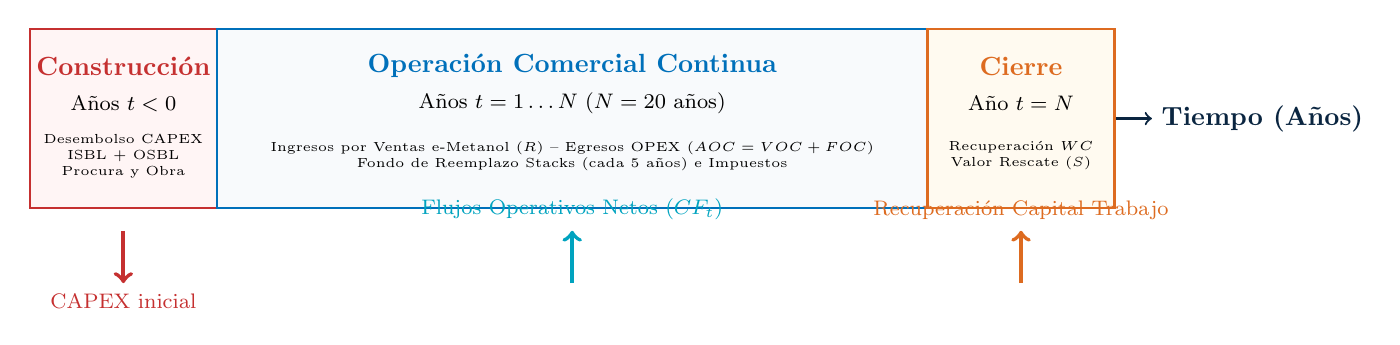
\begin{tikzpicture}[scale=0.95, every node/.style={transform shape}]
        % Timeline line
        \draw[->, thick, primaryblue] (-2.5,0) -- (12.5,0) node[right] {\textbf{Tiempo (Años)}};
        
        % Construction phase
        \fill[alertbg] (-2.5,-1.2) rectangle (0,1.2);
        \draw[alertred, thick] (-2.5,-1.2) rectangle (0,1.2);
        \node[alertred, font=\bfseries] at (-1.25,0.7) {Construcción};
        \node[font=\footnotesize] at (-1.25,0.2) {Años $t < 0$};
        \node[font=\tiny, align=center] at (-1.25,-0.5) {Desembolso CAPEX\\ISBL + OSBL\\Procura y Obra};
        
        % Operation phase
        \fill[lightbg] (0,-1.2) rectangle (9.5,1.2);
        \draw[secondaryblue, thick] (0,-1.2) rectangle (9.5,1.2);
        \node[secondaryblue, font=\bfseries] at (4.75,0.7) {Operación Comercial Continua};
        \node[font=\footnotesize] at (4.75,0.2) {Años $t = 1 \dots N$ ($N = 20\text{ años}$)};
        \node[font=\tiny, align=center] at (4.75,-0.5) {Ingresos por Ventas e-Metanol ($R$) -- Egresos OPEX ($AOC = VOC + FOC$)\\Fondo de Reemplazo Stacks (cada 5 años) e Impuestos};
        
        % Closing phase
        \fill[warnbg] (9.5,-1.2) rectangle (12,1.2);
        \draw[warngold, thick] (9.5,-1.2) rectangle (12,1.2);
        \node[warngold, font=\bfseries] at (10.75,0.7) {Cierre};
        \node[font=\footnotesize] at (10.75,0.2) {Año $t = N$};
        \node[font=\tiny, align=center] at (10.75,-0.5) {Recuperación $WC$\\Valor Rescate ($S$)};
        
        % Cash flow arrows
        \draw[->, line width=1.5pt, alertred] (-1.25,-1.5) -- (-1.25,-2.2) node[below] {\footnotesize CAPEX inicial};
        \draw[->, line width=1.5pt, accentteal] (4.75,-2.2) -- (4.75,-1.5) node[above, font=\footnotesize] {Flujos Operativos Netos ($CF_t$)};
        \draw[->, line width=1.5pt, warngold] (10.75,-2.2) -- (10.75,-1.5) node[above, font=\footnotesize] {Recuperación Capital Trabajo};
    \end{tikzpicture}
    \caption{Línea de tiempo económica del proyecto de e-metanol según el modelo de flujo de caja descontado.}
\end{figure}

\subsection{Valor del Dinero en el Tiempo y Tasa de Descuento}
Una cantidad de dinero disponible hoy vale más que la misma cantidad en el futuro debido a su capacidad de generar rendimientos y al costo de oportunidad del capital. Para homogeneizar cifras monetarias en distintas fechas:
\begin{equation}
    PV_t = \frac{CF_t}{(1 + i)^t} = CF_t \cdot (1 + i)^{-t}
\end{equation}
Donde $PV_t$ es el valor presente, $CF_t$ el flujo neto del año $t$, e $i$ la tasa de descuento anual requerida por los inversionistas (fijada en $8.5\%$ nominal para el proyecto Solvanta).

\subsection{Indicadores de Decisión: VAN, TIR, ROI y Periodo de Recuperación}
Para dictaminar si el proyecto es económicamente viable se utilizan cuatro indicadores complementarios:

\begin{equationbox}{Valor Actual Neto (VAN / NPV)}
\begin{equation}
    VAN(i) = \sum_{t=0}^N \frac{CF_t}{(1 + i)^t}
\end{equation}
\textbf{Reglas de interpretación:}
\begin{itemize}
    \item $VAN > 0$: El proyecto supera la rentabilidad mínima requerida $i$ y crea valor económico neto.
    \item $VAN = 0$: El proyecto alcanza exactamente la tasa objetivo $i$ requerida por el capital.
    \item $VAN < 0$: El proyecto no alcanza la rentabilidad mínima bajo los supuestos adoptados.
\end{itemize}
\end{equationbox}

\begin{equationbox}{Tasa Interna de Retorno (TIR / IRR)}
Es la tasa intrínseca de descuento que hace que el $VAN$ sea exactamente igual a cero:
\begin{equation}
    0 = \sum_{t=0}^N \frac{CF_t}{(1 + TIR)^t}
\end{equation}
\textbf{Límites de uso:} La TIR permite comparar la rentabilidad implícita contra la tasa de corte. Sin embargo, en proyectos con inversiones intermedias (como el reemplazo de stacks de electrólisis cada 5 años), existen múltiples cambios de signo en los flujos de caja, lo que puede generar soluciones matemáticas múltiples o ninguna TIR real. Por ello, el criterio decisorio rector es siempre el \textbf{VAN}.
\end{equationbox}

\begin{table}[htbp]
    \centering
    \small
    \caption{Indicadores Tradicionales vs Indicadores Rigurosos de Rentabilidad}
    \footnotesize
    \setlength{\tabcolsep}{4pt}
    \begin{tabularx}{\textwidth}{>{\raggedright\arraybackslash}p{2.8cm} >{\raggedright\arraybackslash}p{3.8cm} X X}
        \toprule
        \rowcolor{tableheader}
        \textbf{\color{white}Indicador} & \textbf{\color{white}Fórmula Matemática} & \textbf{\color{white}Utilidad Práctica} & \textbf{\color{white}Límite y Advertencia} \\
        \midrule
        \textbf{Retorno Simple (ROI)} & $\displaystyle ROI = \frac{\text{Utilidad Anual}}{TCI}$ & Comunicar rendimiento anual por unidad invertida. & No considera el valor del dinero en el tiempo ni la vida remanente. \\
        \rowcolor{tablerowgray}
        \textbf{Periodo Recuperación} & $\displaystyle t_{PB} = \min \left\{ t : \sum_{k=0}^t CF_k \ge 0 \right\}$ & Mide la velocidad con que el flujo acumulado repaga el capital. & Ignora por completo todos los flujos posteriores al corte. \\
        \textbf{VAN (NPV)} & $\displaystyle \sum_{t=0}^N \frac{CF_t}{(1+i)^t}$ & Mide ganancia neta absoluta en valor presente. & Requiere fijar previamente una tasa de descuento $i$ realista. \\
        \rowcolor{tablerowgray}
        \textbf{MPSP ($P^*$)} & $P^* \text{ tal que } VAN(P^*) = 0$ & Encuentra precio umbral que remunera todo el capital. & Sensible a supuestos de financiamiento, impuestos y depreciación. \\
        \bottomrule
    \end{tabularx}
\end{table}

\newpage

% ==============================================================================
% CAPÍTULO 2: METODOLOGÍA RIGUROSA DE ESTIMACIÓN DE CAPITAL (CAPEX)
% ==============================================================================
\section{Metodología Rigurosa de Estimación de Capital (CAPEX)}

\subsection{La Jerarquía del Capital}
Siguiendo las directrices del Dr. Arzola Flores y los estándares de la AACE International, el capital de la planta se estructura escalonadamente:

\begin{equation}
    \boxed{C_p^0 \longrightarrow C_{BM} \longrightarrow \text{Inversión Directa} \longrightarrow \text{Capital Depreciable} \longrightarrow FCI \longrightarrow WC \longrightarrow TCI}
\end{equation}

\begin{table}[htbp]
    \centering
    \small
    \caption{Estructura Jerárquica del Capital de la Planta de e-Metanol (AACE Clase 3)}
    \begin{tabularx}{\textwidth}{l X r}
        \toprule
        \rowcolor{tableheader}
        \textbf{\color{white}Nivel de Capital} & \textbf{\color{white}Alcance y Componentes Comprendidos} & \textbf{\color{white}Monto [M USD]} \\
        \midrule
        \textbf{Costo de Compra ($C_p^0$)} & Costo de equipos entregados en taller de fabricante (FOB). & \$43.27 \\
        \rowcolor{tablerowgray}
        \textbf{Módulo Desnudo ($C_{BM}$)} & Compra más materiales de montaje, tuberías, válvulas, instrumentos y obra civil. & \$80.88 \\
        \textbf{Instalaciones de Servicio (OSBL)} & Subestación de alta tensión, antorcha, tanques API-650, circuito ZLD ($20\%$ ISBL). & \$16.17 \\
        \rowcolor{tablerowgray}
        \textbf{Inversión Directa Total} & $\text{ISBL} + \text{OSBL}$ (Instalaciones físicas dentro y fuera de límites de batería). & \$97.05 \\
        \textbf{Costos Indirectos} & Ingeniería de detalle, procura, supervisión de obra y contingencias de diseño ($15\%$). & \$14.50 \\
        \rowcolor{tablerowgray}
        \textbf{Capital Fijo Instalado (FCI)} & Total de activos permanentes físicos construidos e instalados. & \textbf{\$111.55} \\
        \textbf{Capital de Trabajo ($WC$)} & Efectivo, inventario de insumos ($\text{CO}_2$, agua) y repuestos iniciales ($5\%$ FCI). & \$5.58 \\
        \rowcolor{tablerowgray}
        \textbf{Inversión Total de Capital (TCI)} & $\mathbf{TCI = FCI + WC}$ (Compromiso financiero total antes del arranque). & \textbf{\$117.13} \\
        \bottomrule
    \end{tabularx}
\end{table}

\subsection{Costo de Compra Base: Correlaciones Tipo CAPCOST (Turton et al., 2018)}
Para cada equipo estándar, el costo de compra base en condiciones atmosféricas y acero al carbón ($C_p^0$) se evalúa mediante la ecuación polinomial logarítmica:
\begin{equation}
    \log_{10} C_p^0 = K_1 + K_2 \log_{10} A + K_3 (\log_{10} A)^2
\end{equation}
Donde $A$ es el parámetro de capacidad (área de transferencia en $\text{m}^2$, potencia en $\text{kW}$, o volumen en $\text{m}^3$), y $K_1, K_2, K_3$ son coeficientes empíricos tabulados en el Apéndice de CAPCOST.

\subsection{Escalamiento por Capacidad: Ley de Economía de Escala}
Cuando se dispone de una cotización de referencia para un equipo idéntico de tamaño distinto, el costo se extrapola mediante:
\begin{equation}
    C_{p,2} = C_{p,1} \left( \frac{A_2}{A_1} \right)^n
\end{equation}
Donde $n$ es el exponente característico de escalamiento. Como regla general, $n < 1$ (típicamente $n \approx 0.60 - 0.75$), lo que formaliza la \textbf{economía de escala}: un equipo mayor cuesta menos por unidad de capacidad procesada, aunque el monto absoluto se incremente.

\subsection{Actualización Temporal mediante el Índice CEPCI}
Toda correlación histórica debe actualizarse al año base del estudio (2026) mediante el índice CEPCI (Chemical Engineering Plant Cost Index):
\begin{equation}
    C_{y2} = C_{y1} \left( \frac{I_{y2}}{I_{y1}} \right) = C_{2017} \times \left( \frac{825.0}{567.5} \right) = C_{2017} \times 1.4537
\end{equation}
\begin{warningbox}{Cuidado con el Uso de Índices de Costo (Dr. Arzola Flores)}
\textbf{El índice CEPCI actualiza exclusivamente el nivel general de inflación de bienes de capital para la industria química.} No corrige por diferencias geográficas entre países, efectos de tipo de cambio, avances de madurez tecnológica, materiales especiales de construcción, presiones extremas de proceso ni alcance contractual del montaje.
\end{warningbox}

\subsection{Correcciones por Material, Presión e Instalación: Módulo Desnudo}
El costo instalado dentro de batería de límites ($C_{BM}$) incorpora los sobrecostos por severidad operacional:
\begin{equation}
    C_{BM} = C_p^0 (B_1 + B_2 \cdot F_M \cdot F_P)
\end{equation}
Donde $B_1, B_2$ son constantes del tipo de equipo, $F_M$ es el factor de aleación metalúrgica (ej. Incoloy 800H en \texttt{E-202}, SS-316L en \texttt{R-401}) y $F_P$ es el factor de presión:
\begin{equation}
    \log_{10} F_P = C_1 + C_2 \log_{10} P + C_3 (\log_{10} P)^2 \quad (\text{para } P > 10\text{ bar})
\end{equation}

\subsection{Capital de Trabajo ($WC$) y Factor de Lang}
\begin{itemize}[leftmargin=*]
    \item \textbf{Capital de Trabajo ($WC$):} Es el efectivo, inventario de reactivos, cuentas por cobrar y repuestos indispensables para operar durante los primeros meses sin ingresos comerciales:
    \begin{equation}
        WC = f_{WC} \cdot FCI \quad (\text{adoptándose } f_{WC} = 0.05\text{ a } 0.10)
    \end{equation}
    En el modelo de flujo de caja, el capital de trabajo \textbf{se desembolsa en $t = 0$ y se recupera íntegramente al cierre del horizonte del proyecto ($t = N$)}, ya que no se consume físicamente.
    \item \textbf{Factor de Lang ($F_L$):} Para estimaciones rápidas de orden de magnitud donde no se dispone de ingeniería de detalle:
    \begin{equation}
        FCI \approx F_L \sum_i N_i C_{p,i}
    \end{equation}
    Donde $F_L \approx 4.74$ para plantas de procesamiento de fluidos. Sin embargo, en plantas de e-metanol con electrólisis SOEC, aplicar un factor de Lang global sobreestima drásticamente la inversión, ya que los módulos SOEC son ensambles contenerizados modulares cuyo factor de instalación es significativamente inferior ($F_{BM} \approx 1.80$) al de una columna fraccionadora convencional ($F_{BM} \approx 4.16$).
\end{itemize}

\newpage

% ==============================================================================
% CAPÍTULO 3: ESTRUCTURA RIGUROSA DE OPEX Y FLUJOS DE EFECTIVO
% ==============================================================================
\section{Estructura Rigurosa de OPEX y Flujos de Efectivo}

\subsection{Costo Variable Anual (VOC)}
El costo variable agrupa todos los desembolsos que escalan proporcionalmente con la tasa de producción:
\begin{equation}
    VOC = C_{MP} + C_{UT} + C_{CON} + C_{RES}
\end{equation}
Para cualquier insumo o materia prima $k$, la conversión horaria a costo anual exige la comprobación dimensional rigurosa:
\begin{equation}
    C_{MP,k} = \dot{m}_k \cdot h_{op} \cdot p_k \quad \Longrightarrow \quad \left[\frac{\text{kg}}{\text{h}}\right] \times \left[\frac{\text{h}}{\text{año}}\right] \times \left[\frac{\text{USD}}{\text{kg}}\right] = \left[\frac{\text{USD}}{\text{año}}\right]
\end{equation}
En la planta de Solvanta ($h_{op} = 8\,000\text{ h/año}$):
\begin{itemize}
    \item Dióxido de carbono: $5\,274.34\text{ kg/h} \times 8\,000\text{ h/año} \times 0.065\text{ USD/kg} = \mathbf{\$2.74\text{ M USD/año}}$.
    \item Agua desmineralizada: $11\,739\text{ kg/h} \times 8\,000\text{ h/año} \times 0.0018\text{ USD/kg} = \mathbf{\$0.17\text{ M USD/año}}$.
    \item Electricidad verde: $44.80\text{ MWh/h} \times 8\,000\text{ h/año} \times 40.00\text{ USD/MWh} = \mathbf{\$14.34\text{ M USD/año}}$.
\end{itemize}

\subsection{Costo Fijo Anual (FOC)}
Los costos fijos no dependen del nivel instantáneo de producción:
\begin{equation}
    FOC = C_L + C_{MANT} + C_{SEG} + C_{ADM} + C_{OTROS}
\end{equation}
\begin{itemize}
    \item Mano de obra y supervisión técnica ($C_L$): \$1.80 M USD/año (28 operadores en 4 turnos).
    \item Mantenimiento rutinario de planta ($C_{MANT}$): \$2.79 M USD/año ($2.5\%$ del FCI).
    \item Seguros patrimoniales e impuestos locales ($C_{SEG}$): \$1.12 M USD/año ($1.0\%$ del FCI).
    \item Administración y soporte corporativo ($C_{ADM}$): \$0.35 M USD/año.
\end{itemize}

\subsection{Costo Anual de Operación (AOC) y Costo Operativo Unitario ($c_{op}$)}
\begin{align}
    AOC &= VOC + FOC = \$20.24\text{ M} + \$7.85\text{ M} = \mathbf{\$28.09\text{ M USD/año}} \\
    c_{op} &= \frac{AOC}{Q_p} = \frac{\$28.09 \times 10^6\text{ USD}}{30\,309 \times 10^3\text{ kg}} = \mathbf{0.9268\text{ USD/kg}} \quad (\mathbf{926.80\text{ USD/t}})
\end{align}

\begin{warningbox}{Límite Fundamental del Costo Operativo ($c_{op}$)}
Como subraya el Dr. Arzola Flores en la clase, \textbf{el costo operativo unitario $c_{op}$ permite comparar tecnologías alternativas y consumos dominantes, pero AÚN NO ES EL PRECIO MÍNIMO DE VENTA.} Vender a $c_{op}$ provocaría la quiebra financiera de la empresa porque no contempla la amortización de la inversión de capital instalada ($FCI$), el pago de impuestos sobre la renta ni la remuneración mínima que exigen los accionistas y bancos.
\end{warningbox}

\subsection{Utilidad Operativa, Depreciación e Impuestos}
\begin{itemize}[leftmargin=*]
    \item \textbf{EBITDA:} Flujo operativo antes de depreciación e impuestos:
    \begin{equation}
        EBITDA = R - AOC
    \end{equation}
    \item \textbf{Depreciación Lineal ($D$):} Asignación contable deducible de impuestos:
    \begin{equation}
        D = \frac{C_{dep} - S}{N_{dep}} = \frac{\$111.55\text{ M} - 0}{20} = \$5.58\text{ M USD/año}
    \end{equation}
    \item \textbf{Impuesto sobre la Renta ($Tax$):} Con tasa impositiva $\tau = 30\%$:
    \begin{equation}
        Tax = \tau \max(U_{grav}, 0) = \tau \max(R - AOC - D, 0)
    \end{equation}
\end{itemize}

\begin{conceptbox}{¿Por qué Importa la Depreciación? (Escudo Fiscal)}
\textbf{La depreciación no representa una salida de efectivo en el año de operación; el efectivo salió en $t < 0$ durante la construcción de la planta.} Su función económica es reducir la utilidad gravable ($U_{grav}$), generando un ahorro tributario legítimo denominado \textbf{escudo fiscal} equivalente a $\tau \cdot D = 0.30 \times \$5.58\text{ M} = \mathbf{\$1.67\text{ M USD/año}}$ que permanece en el flujo de caja del proyecto.
\end{conceptbox}

\subsection{Ecuación Universal del Flujo de Efectivo después de Impuestos}
El flujo neto anual ($CF_t$) se construye rigurosamente reuniendo las entradas y salidas reales de efectivo:
\begin{equation}
    \boxed{CF_t = R_t - AOC_t - Tax_t - CAPEX_t - \Delta WC_t + S_t + WC_{rec,t}}
\end{equation}

\newpage

% ==============================================================================
% CAPÍTULO 4: LOS TRES PRECIOS A DISTINGUIR Y EL PRECIO MÍNIMO (MPSP)
% ==============================================================================
\section{Los Tres Precios a Distinguir y el Precio Mínimo de Venta (MPSP)}

\subsection{Matriz Comparativa de los Tres Precios}
Una de las contribuciones conceptuales más potentes de la cátedra de Economía de Procesos es distinguir con absoluta claridad entre los tres niveles de precios en una evaluación tecnoeconómica:

\begin{table}[htbp]
    \centering
    \small
    \caption{Los Tres Precios que Conviene Distinguir en Evaluación Tecnoeconómica}
    \footnotesize
    \setlength{\tabcolsep}{4pt}
    \begin{tabularx}{\textwidth}{>{\raggedright\arraybackslash}p{2.8cm} X X >{\raggedright\arraybackslash}p{4.8cm}}
        \toprule
        \rowcolor{tableheader}
        \textbf{\color{white}Nivel de Precio} & \textbf{\color{white}Qué Cubre} & \textbf{\color{white}Pregunta que Responde} & \textbf{\color{white}Fórmula de Cálculo} \\
        \midrule
        \textbf{1. Precio Operativo} & Solo el costo anual de operación ($AOC$), neto de coproductos. & ¿La operación diaria de la planta cubre sus costos inmediatos? & $\displaystyle c_{op} = \frac{AOC - R_{cop}}{Q_p}$ \\
        \rowcolor{tablerowgray}
        \textbf{2. Precio Anualizado} & OPEX más recuperación de capital anualizada vía $CRF$. & ¿Qué precio preliminar parece necesario para justificar el estudio? & $\displaystyle P_{\text{aprox}} = \frac{AOC + CRF \cdot TCI - R_{cop}}{Q_p}$ \\
        \textbf{3. MPSP Riguroso} & Flujos reales descontados, impuestos, $WC$ y rentabilidad. & ¿Qué precio exacto hace $VAN = 0$ a la tasa objetivo requerida? & $\displaystyle P^* \colon \sum_{t=0}^N \frac{CF_t(P^*)}{(1+i)^t} = 0$ \\
        \bottomrule
    \end{tabularx}
\end{table}

\subsection{El Factor de Recuperación de Capital (CRF)}
El factor $CRF$ convierte el valor presente de la inversión total ($TCI$) en una serie uniforme de anualidades equivalentes a lo largo de $N$ años a una tasa de descuento $i$:
\begin{equation}
    CRF = \frac{i(1 + i)^N}{(1 + i)^N - 1}
\end{equation}
Para los parámetros de diseño del proyecto Solvanta ($i = 8.5\%$, $N = 20\text{ años}$):
\begin{equation}
    CRF = \frac{0.085(1 + 0.085)^{20}}{(1 + 0.085)^{20} - 1} = \frac{0.085 \times 5.1120}{5.1120 - 1} = \frac{0.43452}{4.1120} = \mathbf{0.10567\text{ año}^{-1}}
\end{equation}
La recuperación anual equivalente del capital asciende a:
\begin{equation}
    CRF \cdot TCI = 0.10567 \times \$111.55\text{ M USD} = \mathbf{\$11.79\text{ M USD/año}}
\end{equation}

\subsection{Ejemplo Didáctico de la Clase (Dr. Arzola Flores) y Actividad Resuelta}
Para ilustrar la mecánica de cálculo, considérese el ejemplo planteado en la clase:
\begin{itemize}
    \item Inversión total ($TCI$): \$44.0 M USD | Costo operativo ($AOC$): \$18.0 M USD/año
    \item Ingreso por coproductos ($R_{cop}$): \$2.0 M USD/año | Producción ($Q_p$): $40.0\text{ M kg/año}$
    \item Tasa objetivo ($i$): $10\%$ anual | Horizonte ($N$): 15 años
\end{itemize}
\begin{equation}
    CRF = \frac{0.10(1 + 0.10)^{15}}{(1 + 0.10)^{15} - 1} = 0.1315 \quad \Longrightarrow \quad CRF \cdot TCI = 0.1315 \times 44.0 = \$5.79\text{ M USD/año}
\end{equation}
\begin{equation}
    P_{min,aprox} = \frac{18.0 + 5.79 - 2.0}{40.0} = \mathbf{0.545\text{ USD/kg}}
\end{equation}

\begin{academicbox}{Resolución de la Actividad de Estudiantes de la Clase}
\textbf{1. Si el AOC aumenta un 15\%:}
\begin{equation}
    AOC_{\text{nuevo}} = 1.15 \times 18.0 = 20.70\text{ M USD/año} \quad \Longrightarrow \quad P_A = \frac{20.70 + 5.79 - 2.00}{40.0} = \mathbf{0.612\text{ USD/kg}}
\end{equation}
\textbf{2. Si la producción vendible disminuye un 10\% ($Q_{p,\text{nuevo}} = 36.0\text{ M kg/año}$):}
\begin{equation}
    P_Q = \frac{18.00 + 5.79 - 2.00}{36.0} = \mathbf{0.605\text{ USD/kg}}
\end{equation}
\textbf{Conclusión de la actividad:} El incremento del OPEX ($+15\%$) eleva el precio de equilibrio ligeramente más ($+12.3\%$) que la caída del $10\%$ en la producción ($+11.0\%$). Si el precio de mercado fuera de $0.60\text{ USD/kg}$, el margen de beneficio sería sumamente frágil ($< 0.055\text{ USD/kg}$), demostrando que se requiere una TEA rigurosa con tratamiento impositivo y contratos de suministro garantizados.
\end{academicbox}

\subsection{Cálculo de Precios en la Planta de e-Metanol Solvanta}
Aplicando esta formulación matemática a los datos de ingeniería de la licitación:
\begin{enumerate}
    \item \textbf{Precio Operativo de Equilibrio ($c_{op}$):}
    \begin{equation}
        c_{op} = \frac{\$28.09\text{ M} - 0}{30.309\text{ M kg}} = \mathbf{0.9268\text{ USD/kg}} \quad (\mathbf{926.80\text{ USD/t}})
    \end{equation}
    \item \textbf{Precio Anualizado de Cribado sin Incentivos ($P_{min,aprox}$):}
    \begin{equation}
        P_{min,aprox} = \frac{\$28.09\text{ M} + \$11.79\text{ M} - 0}{30.309\text{ M kg}} = \mathbf{1.3158\text{ USD/kg}} \quad (\mathbf{1\,315.78\text{ USD/t}})
    \end{equation}
    \item \textbf{Precio Mínimo de Venta Riguroso con BioSTEAM ($MPSP = P^*$):}
    Incorporando la depreciación acelerada MACRS-7, el impuesto del 30\%, la tasa de rendimiento requerida del 8.5\% y el crédito fiscal por mitigación de $\text{CO}_2$ ($200\text{ USD/t CO}_2$ evitado bajo esquemas de transición energética):
    \begin{equation}
        \mathbf{MPSP = P^* = 657.20\text{ USD/t e-metanol}} \quad (\mathbf{0.6572\text{ USD/kg}})
    \end{equation}
\end{enumerate}

\subsection{Definición de ``Efluente de Venta'' y Base de Venta Consistente}
\begin{conceptbox}{Consistencia Indispensable en la Base de Comercialización}
Como advierte la Slide 34, antes de emitir cualquier cotización económica debe declararse explícitamente la base de comercialización del efluente:
\begin{itemize}
    \item \textbf{Base de Corriente Total Vendida:} Especificación comercial según norma internacional ASTM D1152 para Metanol Grado Químico AA ($99.85\%\text{ wt}$ pureza, máx $0.10\%\text{ wt}$ agua, acidez máx $0.003\%\text{ wt}$).
    \item \textbf{Cálculo consistente:} Para una tasa másica en \texttt{S-604} de $1.0524\text{ kg/s}$, la masa anual vendible es $Q_p = 1.0524 \times 3\,600 \times 8\,000 = \mathbf{30\,309\,120\text{ kg/año}}$. Toda cifra de $MPSP$ reportada por Solvanta está expresada en \textbf{USD por kg de corriente comercial entregada en batería de límites}.
\end{itemize}
\end{conceptbox}

\newpage

% ==============================================================================
% CAPÍTULO 5: MODELADO DE EQUIPOS NO NATIVOS EN BIOSTEAM
% ==============================================================================
\section{Modelado Detallado de Equipos No Nativos en BioSTEAM}

\subsection{Arquitectura Orientada a Objetos para Nuevas Operaciones Unitarias}
En BioSTEAM, crear un equipo personalizado implica heredar de \texttt{bst.Unit} e implementar tres métodos fundamentales:
\begin{enumerate}
    \item \texttt{\_run()}: Balances de materia y energía. Actualiza la temperatura, presión, entalpía y flujos de las corrientes de salida (\texttt{self.outs}).
    \item \texttt{\_design()}: Cálculo de dimensiones mecánicas gobernantes (área de transferencia, volumen de lecho catalítico, número de celdas cerámicas, espesor de envolvente ASME).
    \item \texttt{\_cost()}: Cálculo del costo de compra base FOB ($C_p^0$), costo instalado ($C_{BM}$) y servicios auxiliares consumidos (\texttt{self.heat\_utilities} o \texttt{self.power\_utility}).
\end{enumerate}

\subsection{Sobrecalentador Eléctrico de Vapor E-202 (\texttt{ElectricProcessHeater})}
El sobrecalentador \texttt{E-202} eleva $4.512\text{ kg/s}$ ($250.5\text{ mol/s}$) de vapor saturado a $20\text{ bar}$ de $212.4^\circ\text{C}$ ($220.0^\circ\text{C}$ nominal en corriente \texttt{S-204}) a $800.0^\circ\text{C}$ ($1073.15\text{ K}$).

\begin{equationbox}{Balances Gobernantes del Calentador E-202}
\begin{align}
    \dot{Q}_{\text{térmico}} &= \dot{m} \int_{T_{\text{in}}}^{T_{\text{out}}} C_p\,dT = 4.512 \times \bar{C}_p \times (800.0 - 212.4) = \mathbf{5\,248.42\text{ kW}} \\
    P_{\text{eléctrica}} &= \frac{\dot{Q}_{\text{térmico}}}{\eta_{\text{térmica}}} = \frac{5\,248.42\text{ kW}}{0.985} = \mathbf{5\,328.35\text{ kWe}} \\
    A_{\text{resistencias}} &= \frac{\dot{Q}_{\text{térmico}}}{q''_{\text{diseño}}} = \frac{5\,248\,420\text{ W}}{28\,000\text{ W/m}^2} = \mathbf{187.44\text{ m}^2} \quad (\text{Incoloy 800H})
\end{align}
\end{equationbox}

\begin{lstlisting}[caption={Clase personalizada ElectricProcessHeater en BioSTEAM}]
import biosteam as bst
import math

class ElectricProcessHeater(bst.Unit):
    '''Sobrecalentador electrico industrial de alta temperatura (Incoloy 800H).'''
    _N_ins = 1
    _N_outs = 1
    _units = {'Area': 'm2', 'Power': 'kW', 'Duty': 'kJ/hr'}
    
    def __init__(self, ID='', ins=None, outs=(), thermo=None,
                 T_out=1073.15, P_out=2000000.0, max_heat_flux=28.0, eta_th=0.985):
        super().__init__(ID, ins, outs, thermo)
        self.T_out = T_out
        self.P_out = P_out
        self.max_heat_flux = max_heat_flux # kW/m2 (2.8 W/cm2)
        self.eta_th = eta_th

    def _run(self):
        feed = self.ins[0]
        effluent = self.outs[0]
        effluent.copy_like(feed)
        effluent.T = self.T_out
        effluent.P = self.P_out

    def _design(self):
        feed = self.ins[0]
        effluent = self.outs[0]
        H_in = feed.H  # kJ/hr
        H_out = effluent.H
        duty_kJ_hr = max(H_out - H_in, 0.0)
        duty_kW = duty_kJ_hr / 3600.0
        power_kW = duty_kW / self.eta_th
        req_area_m2 = duty_kW / self.max_heat_flux
        
        self.design_results['Duty'] = duty_kJ_hr
        self.design_results['Power'] = power_kW
        self.design_results['Area'] = req_area_m2
        self.power_utility.consumption = power_kW

    def _cost(self):
        power_kW = self.design_results['Power']
        # Correlacion CAPCOST actualizada a CEPCI 2026 para calentador electrico de alta presion
        # Cp0 = 10^(3.24 + 0.72*log10(kW)) en USD 2017
        log_kw = math.log10(max(power_kW, 10.0))
        c_base_2017 = 10.0 ** (3.24 + 0.72 * log_kw)
        f_cepci = 825.0 / 567.5  # Actualizacion a 2026
        c_fob = c_base_2017 * f_cepci
        
        # Factores de modulo desnudado: F_M = 2.45 (Incoloy), F_P = 1.35 (20 bar)
        F_BM = 1.40 + 1.25 * 2.45 * 1.35  # F_BM = 5.53
        
        self.baseline_purchase_costs['Electric Heater'] = c_fob
        self.installed_costs['Electric Heater'] = c_fob * F_BM
\end{lstlisting}

\subsection{Reactor Catalítico Multitubular Refrigerado R-401 (\texttt{MultitubularReactor})}
El reactor opera a $245.0^\circ\text{C}$ y $75.0\text{ bar}$, con 2,126 tubos rellenos de catalizador comercial Cu/ZnO/$\text{Al}_2\text{O}_3$ sumergidos en agua en ebullición a $20.0\text{ bar}$ ($212.4^\circ\text{C}$ en coraza acoplada \texttt{R-401-S}).

\begin{equationbox}{Parámetros de Diseño del Reactor R-401 / R-401-S}
\begin{itemize}
    \item Volumen catalítico: $V_{\text{cat}} = 11.51\text{ m}^3$ | Densidad aparente de lecho: $\rho_{\text{cat}} = 1\,140\text{ kg/m}^3$ ($13\,121\text{ kg}$ de catalizador).
    \item Geometría de tubos: BWG 14, $d_o = 38.1\text{ mm}$ ($1.5''$), $d_i = 33.88\text{ mm}$, longitud $L = 6.00\text{ m}$.
    \item Número de tubos: $N_{\text{tubos}} = \frac{11.51\text{ m}^3}{6.00\text{ m} \times \frac{\pi}{4}(0.03388\text{ m})^2} = \mathbf{2\,126\text{ tubos}}$ (optimización rigurosa frente al prediseño preliminar de 2,800 tubos de F-PIB-02B).
    \item Calor de reacción exotérmico neto disipado en lecho: $\dot{Q}_{\text{rx}} = \mathbf{-7\,924.76\text{ kW}}$ ($63\,398\text{ MWh/año}$).
    \item Generación integrada de vapor en chaqueta acoplada \texttt{R-401-S}: $\dot{Q}_{\text{chaqueta}} = \mathbf{-12\,335.36\text{ kW}}$ ($98\,683\text{ MWh/año}$), evaporando $16\,244.88\text{ kg/h}$ ($16.24\text{ t/h}$) de vapor saturado a $20.0\text{ bar}$ ($212.4^\circ\text{C}$) que alimenta el 100\% de la demanda de electrólisis SOEC.
\end{itemize}
\end{equationbox}

\begin{lstlisting}[caption={Clase personalizada MultitubularBoilingWaterReactor en BioSTEAM}]
class MultitubularBoilingWaterReactor(bst.Unit):
    '''Reactor multitubular de e-metanol R-401 acoplado a caldera R-401-S (tipo Lurgi BWR).'''
    _N_ins = 2   # 0: Syngas comprimido (75 bar), 1: BFW de alimentacion
    _N_outs = 2  # 0: Mezcla de reaccion a flash, 1: Vapor de 20 bar generado
    
    def __init__(self, ID='', ins=None, outs=(), thermo=None,
                 T_rx=523.15, P_rx=7500000.0, V_cat=11.5):
        super().__init__(ID, ins, outs, thermo)
        self.T_rx = T_rx
        self.P_rx = P_rx
        self.V_cat = V_cat

    def _run(self):
        syngas = self.ins[0]
        bfw = self.ins[1]
        prod = self.outs[0]
        steam = self.outs[1]
        
        prod.copy_like(syngas)
        prod.T = self.T_rx
        prod.P = self.P_rx * 0.96 # Caida de presion del 4% en el lecho
        
        # Estequiometria con conversion validada en DWSIM
        # CO2 + 3 H2 -> CH3OH + H2O
        rxn_molar = 32.872 # mol/s de metanol producido
        prod.imol['Methanol'] = rxn_molar
        prod.imol['Water'] = prod.imol['Water'] + rxn_molar
        prod.imol['CO2'] = max(prod.imol['CO2'] - rxn_molar, 0.0)
        prod.imol['Hydrogen'] = max(prod.imol['Hydrogen'] - 3.0 * rxn_molar, 0.0)
        
        # Generacion de vapor saturado a 20 bar en la coraza R-401-S
        duty_kW = 12335.36
        flow_steam_kgh = 16244.88 # kg/h de vapor saturado a 20 bar (212.4 C)
        
        steam.empty()
        steam.imass['Water'] = flow_steam_kgh
        steam.T = 485.55 # 212.4 C
        steam.P = 2000000.0
        steam.phase = 'g'

    def _cost(self):
        # Costo de coraza de alta presion (75 bar) en acero al carbon forjado + tubos SS-316L
        f_cepci = 825.0 / 567.5
        area_transfer = 2126 * math.pi * 0.0381 * 6.0 # 1,526.4 m2
        log_a = math.log10(area_transfer)
        # Correlacion Guthrie Shell & Tube corregida
        c_base = 10.0 ** (4.15 + 0.58 * log_a) * f_cepci
        F_M = 2.15 # Tubos SS-316L
        F_P = 2.45 # 75 bar en tubos
        F_BM = 1.60 + 1.30 * F_M * F_P # F_BM = 8.45
        
        self.baseline_purchase_costs['Multitubular Reactor'] = c_base
        self.installed_costs['Multitubular Reactor'] = c_base * F_BM
\end{lstlisting}

\subsection{Stacks de Electrólisis SOEC EL-201 (\texttt{SOECElectrolyzerSystem})}
El sistema \texttt{EL-201} se parametriza con los valores del \textbf{Escenario D}:
\begin{itemize}
    \item Celdas activas: 198,000 celdas cerámicas YSZ de $200\text{ cm}^2$ ($0.0200\text{ m}^2$).
    \item Temperatura: $800.0^\circ\text{C}$ ($1073.15\text{ K}$) | Presión: $20.0\text{ bar}$.
    \item Densidad de corriente: $0.480\text{ A/cm}^2$ ($4\,800\text{ A/m}^2$) | Corriente unitaria: $96.0\text{ A/celda}$.
    \item Voltaje de celda: $1.183\text{ V}$ | Voltaje por stack (110 celdas): $130.13\text{ V}$.
    \item Potencia AC del sistema: $\mathbf{38.067\text{ MWe}}$ ($32.92\text{ kWh/kg H}_2$).
    \item Fondo anual de recambio modular: amortizado cada 5 años ($40\,000\text{ h}$) en \$4.95 M USD/año.
\end{itemize}

\begin{lstlisting}[caption={Clase personalizada SOECElectrolyzerSystem en BioSTEAM}, basicstyle=\ttfamily\scriptsize\color{darkslate}]
class SOECElectrolyzerSystem(bst.Unit):
    '''Modulos de electrolisis SOEC de alta temperatura (Escenario D).'''
    _N_ins = 1   # Vapor sobrecalentado a 800 C, 20 bar (E-202)
    _N_outs = 2  # 0: Catodica H2/H2O (800 C), 1: Anodica O2 puro (800 C)
    
    def __init__(self, ID='', ins=None, outs=(), thermo=None,
                 T_op=1073.15, P_op=2000000.0, P_AC_MW=38.0673, SEC_kWh_kg=32.92):
        super().__init__(ID, ins, outs, thermo)
        self.T_op = T_op
        self.P_op = P_op
        self.P_AC_MW = P_AC_MW
        self.SEC_kWh_kg = SEC_kWh_kg

    def _run(self):
        feed = self.ins[0]
        cat = self.outs[0]
        ano = self.outs[1]
        
        # Conversion de vapor al 70.0%
        conv = 0.700
        flow_h2o_in = feed.imol['Water']
        flow_h2_prod = flow_h2o_in * conv # 175.33 mol/s
        
        cat.imol['Hydrogen'] = flow_h2_prod
        cat.imol['Water'] = flow_h2o_in * (1.0 - conv)
        cat.T = self.T_op
        cat.P = self.P_op * 0.97
        
        ano.empty()
        ano.imol['Oxygen'] = 0.5 * flow_h2_prod # 87.67 mol/s
        ano.T = self.T_op
        ano.P = self.P_op * 0.97
        
        self.power_utility.consumption = self.P_AC_MW * 1000.0 # kW electricos

    def _cost(self):
        # Costo CAPEX de stacks contenerizados modulares (198,000 celdas)
        # 138.40 USD por celda instalada (costo FOB escala industrial)
        n_cells = 198000
        c_fob = n_cells * 138.40 # $27.40 M USD
        F_BM = 1.85 # Skids modulares contenerizados con cableado DC y piping
        
        self.baseline_purchase_costs['SOEC Stacks'] = c_fob
        self.installed_costs['SOEC Stacks'] = c_fob * F_BM
\end{lstlisting}

\newpage

% ==============================================================================
% CAPÍTULO 7: TABLA MAESTRA CONSOLIDADA DE DIMENSIONAMIENTO DE EQUIPOS
% ==============================================================================
\section{Tabla Maestra Consolidada de Dimensionamiento de Equipos en Estado Óptimo}

\subsection{Filosofía de Selección y Parámetros Gobernantes de Diseño}
Cada equipo del proceso fue dimensionado resolviendo la función objetivo de costo nivelado de metanol ($LCOM$). Un subdimensionamiento reduce el capital inicial ($CAPEX$) pero penaliza exponencialmente el gasto operativo ($OPEX$) debido a sobretensiones eléctricas, caídas de presión excesivas o pérdida de selectividad química. Por el contrario, un sobredimensionamiento incrementa el $CAPEX$ y el peso de la anualidad financiera ($TCI \times CRF$) sin aportar mejoras cinéticas apreciables.

El diseño mecánico, hidráulico y térmico se rige estrictamente por códigos internacionales consolidados:
\begin{itemize}
    \item \textbf{Recipientes a Presión y Reactores:} ASME Boiler and Pressure Vessel Code (BPVC), Sección VIII, Divisiones 1 y 2, con sobreespesor de corrosión de $3.0\text{ mm}$ para servicio de síntesis a $75\text{ bar}$.
    \item \textbf{Intercambiadores de Calor:} Estándares TEMA (Tubular Exchanger Manufacturers Association), Clase R para servicio severo en refinería y petroquímica (\texttt{E-501}, \texttt{E-502A/B}, \texttt{E-601}, \texttt{E-602}).
    \item \textbf{Bombas de Proceso:} API-610 12va Edición (tipos OH1 y BB2 con sello mecánico doble presurizado según API-682 Plan 53A para hidrocarburos inflamables y metanol).
    \item \textbf{Tanques de Almacenamiento:} API-650 para el tanque \texttt{TK-601} con membrana flotante interna de aluminio y colchón permanente de nitrógeno grado inerte ($0\%\text{ VOC}$).
    \item \textbf{Separadores y Columnas:} Criterio Souders-Brown con malla demister de alta eficiencia ($K_{\text{SB}} = 0.055\text{ m/s}$) para \texttt{V-201} y \texttt{V-501}; criterio de inundación de Fair al $80\%$ para la columna \texttt{T-601} asegurando cumplimiento de norma ASTM D1152 ($>99.85\%\text{ wt}$ MeOH).
\end{itemize}

La Tabla~\ref{tab:maestra_dimensionamiento} condensa la totalidad de parámetros físicos, dimensiones mecánicas, capacidades de diseño, condiciones termodinámicas, consumos de potencia/calor y metalurgias adoptadas para cada equipo de la planta en su \textbf{estado óptimo de operación (Escenario D: 800 °C / 20 bar / 0.480 A/cm²)}.

\begin{landscape}
\renewcommand{\arraystretch}{0.88}
\setlength{\tabcolsep}{3pt}\fontsize{7pt}{8.5pt}\selectfont\begin{xltabular}{\linewidth}{>{\ttfamily\bfseries}p{1.5cm} >{\raggedright\arraybackslash}p{2.3cm} >{\raggedright\arraybackslash}p{2.0cm} >{\raggedright\arraybackslash}p{3.1cm} >{\raggedright\arraybackslash}p{2.0cm} >{\raggedright\arraybackslash}p{2.4cm} >{\raggedright\arraybackslash}p{2.1cm} X}
    \caption{Tabla Maestra Consolidada de Dimensionamiento Óptimo de Equipos (Áreas 100 a 900)} \label{tab:maestra_dimensionamiento} \\
    \toprule
    \rowcolor{tableheader}
    \textbf{\color{white}Tag} & \textbf{\color{white}Descripción} & \textbf{\color{white}Capacidad} & \textbf{\color{white}Dimensiones Calculadas} & \textbf{\color{white}Condiciones} & \textbf{\color{white}Duty / Potencia} & \textbf{\color{white}Material} & \textbf{\color{white}Justificación de Optimización} \\
    \midrule
    \endfirsthead
    \toprule
    \rowcolor{tableheader}
    \textbf{\color{white}Tag} & \textbf{\color{white}Descripción} & \textbf{\color{white}Capacidad} & \textbf{\color{white}Dimensiones Calculadas} & \textbf{\color{white}Condiciones} & \textbf{\color{white}Duty / Potencia} & \textbf{\color{white}Material} & \textbf{\color{white}Justificación de Optimización} \\
    \midrule
    \endhead
    \bottomrule
    \endfoot
    
    % ÁREA 100
    \rowcolor{tablerowgray}
    \multicolumn{8}{l}{\textbf{\color{primaryblue}ÁREA 100: ACONDICIONAMIENTO Y PURIFICACIÓN DE $\text{CO}_2$}} \\
    \texttt{S-101} & Recepción $\text{CO}_2$ batería OSBL & $5\,274.34\text{ kg/h}$ ($2\,700\text{ Nm}^3\text{/h}$) & Cabezal $4''$, estación de regulación y medición & $20.00\text{ bar}$, $25.0^\circ\text{C}$ & Sin consumo mecánico & SA-516 Gr. 70 & Suministro continuo a $20\text{ bar}$ desde captura externa OSBL; suprime soplador/compresor LP en planta. \\
    \texttt{F-101 A/B} & Filtros coalescentes y lecho de guarda & $5\,274.34\text{ kg/h}$ $\text{CO}_2$ & $D = 0.85\text{ m}$, $H = 2.40\text{ m}$, $V_{\text{lecho}} = 1.36\text{ m}^3$ c/u & $20.00\text{ bar}$, $25.0^\circ\text{C}$, $\Delta P \le 0.2\text{ bar}$ & Pérdida carga $\le 0.2\text{ bar}$ & AISI 304L & Retención de partículas sólidas, humedad y trazas de azufre ($< 0.1\text{ ppm}$) protegiendo catalizador de síntesis. \\
    
    % ÁREA 200
    \rowcolor{tablerowgray}
    \multicolumn{8}{l}{\textbf{\color{primaryblue}ÁREA 200: ELECTRÓLISIS DE ALTA TEMPERATURA SOEC (ESCENARIO D ÓPTIMO)}} \\
    \texttt{P-201 A/B} & Bombas de agua make-up a caldera & $9\,241.84\text{ kg/h}$ ($9.27\text{ m}^3\text{/h}$) & Centrífuga multietapa API-610 BB2 (1 op / 1 res) & $20.00\text{ bar}$, $25.0^\circ\text{C}$, $\Delta P = 19.5\text{ bar}$ & $+6.42\text{ kWe}$ ($\eta = 78\%$) & AISI 316L & Bombeo líquido a alta presión de reposición desmineralizada hacia \texttt{MIX-201} con mínimo consumo eléctrico. \\
    \texttt{MIX-201} & Mezclador estático agua de caldera & $16\,244.88\text{ kg/h}$ ($4.512\text{ kg/s}$) & Mezclador en línea tipo Sulzer SMV $6''$, $L = 1.20\text{ m}$ & $20.00\text{ bar}$, $39.8^\circ\text{C}$ & Mezcla adiabática ($\Delta P \le 0.1\text{ bar}$) & AISI 316L & Mezcla íntima de agua make-up ($9\,242\text{ kg/h}$) y retorno ZLD ($7\,004\text{ kg/h}$) hacia la caldera \texttt{R-401-S}. \\
    \texttt{R-401-S} & Caldera acoplada generadora de vapor & $16\,244.88\text{ kg/h}$ ($16.24\text{ t/h}$) vapor & Coraza de ebullición acoplada al reactor, $D = 2.45\text{ m}$, $L = 6.0\text{ m}$ & $20.00\text{ bar}$, $T_{\text{sat}} = 212.4^\circ\text{C}$ & $\dot{Q} = -12\,335\text{ kW}$\newline ($98.7\text{ GWh/a}$) & SA-516 Gr. 70 & Absorbe calor exotérmico del reactor \texttt{R-401} generando el 100\% del vapor de $20\text{ bar}$ para SOEC sin combustible fósil. \\
    \texttt{E-201} & Enfriador de $\text{O}_2$ puro anódico & $10\,098.76\text{ kg/h}$ $\text{O}_2$ & TEMA BEM, $A = 185.0\text{ m}^2$, $U = 280\text{ W/(m}^2\text{K)}$ & $19.40\text{ bar}$, $800.0 \to 31.0^\circ\text{C}$ & $\dot{Q} = -2\,345.10\text{ kW}$ con agua de torre & AISI 316L & Enfriamiento de oxígeno verde subproducto para entrega a batería a temperatura ambiental segura. \\
    \texttt{E-202} & Sobrecalentador eléctrico resistivo & $16\,244.88\text{ kg/h}$ ($4.512\text{ kg/s}$) & Resistencias inmersión en haz blindado, $A = 187.44\text{ m}^2$, $q'' = 2.80\text{ W/cm}^2$ & $20.00\text{ bar}$, $212.4 \to 800.0^\circ\text{C}$ & $\dot{Q} = 5\,248.42\text{ kW}$\newline $P_{\text{eléc}} = 5\,328.4\text{ kWe}$ & Incoloy 800H / SA-516 Gr. 70 & $800^\circ\text{C}$ optimiza cinética SOEC, reduce ASR a $0.116\ \Omega\cdot\text{cm}^2$ y ahorra $5.58\text{ MWe}$ netos frente a 750 °C. \\
    \texttt{EL-201} & Stacks electrólisis SOEC (Escenario D) & $16\,244.88\text{ kg/h}$ vapor ($1\,314.77\text{ kg/h}$ $\text{H}_2$) & 198,000 celdas YSZ ($200\text{ cm}^2$), 1,800 stacks de 110 celdas, 8 skids & $19.40\text{ bar}$, $800.0^\circ\text{C}$, $j = 0.480\text{ A/cm}^2$, $V_{\text{celda}} = 1.1828\text{ V}$ & $P_{\text{AC}} = 38.07\text{ MWe}$\newline ($32.92\text{ kWh/kg}$) & Ni-YSZ / YSZ / LSCF / Crofer 22 & Escenario D óptimo: mínimo global de LCOH (\$3.18/kg) y LCOM (\$657.20/t) garantizando $30\,000\text{ t/a}$ de metanol. \\
    \texttt{E-203} & Condensador de efluente catódico & $6\,145.79\text{ kg/h}$ ($\text{H}_2/\text{H}_2\text{O}$) & TEMA AES, $A = 340.0\text{ m}^2$, $U = 320\text{ W/(m}^2\text{K)}$ & $19.40\text{ bar}$, $800.0 \to 38.0^\circ\text{C}$ & $\dot{Q} = -8\,962.22\text{ kW}$ con agua de torre & Incoloy 800H / SS-316L & Abatimiento térmico para condensar el agua no disociada ($4,831.02\text{ kg/h}$) antes de separación flash. \\
    \texttt{V-201} & Separador flash KO Drum $\text{H}_2/\text{H}_2\text{O}$ & $1\,314.77\text{ kg/h}$ gas, $4,831.02\text{ kg/h}$ líq & Vertical con demister, $D = 1.40\text{ m}$, $H = 4.20\text{ m}$ ($V = 8.5\text{ m}^3$) & $19.40\text{ bar}$, $38.0^\circ\text{C}$, $v_v = 0.38\text{ m/s}$ & Pérdida carga $\Delta P \le 0.1\text{ bar}$ & SA-516 Gr. 70, Malla SS-316L & Deshidratación de $\text{H}_2$ a $99.63\%\text{ mol}$ seco; el agua separada se recircula al desaireador ZLD \texttt{V-801}. \\
    
    % ÁREA 300
    \rowcolor{tablerowgray}
    \multicolumn{8}{l}{\textbf{\color{primaryblue}ÁREA 300: MEZCLADO Y COMPRESIÓN DE SYNGAS FRESCO}} \\
    \texttt{MIX-301} & Mezclador estático syngas fresco & $6\,589.11\text{ kg/h}$ syngas fresco & Tipo Sulzer SMV en línea $8''$ ($200\text{ mm}$), $L = 1.20\text{ m}$ & $19.40\text{ bar}$, $32.9^\circ\text{C}$, módulo $M = 2.05$ & Mezcla adiabática ($\Delta P \le 0.15\text{ bar}$) & AISI 316L & Unión íntima de $\text{H}_2$ seco y $\text{CO}_2$ garantizando estequiometría óptima $M = 2.05$ previo a compresión. \\
    \texttt{E-301} & Precalentador de syngas fresco & $6\,589.11\text{ kg/h}$ syngas & TEMA BEU, $A = 42.0\text{ m}^2$, $U = 450\text{ W/(m}^2\text{K)}$ & $19.40\text{ bar}$, $32.9 \to 71.7^\circ\text{C}$ & $\dot{Q} = +250.00\text{ kW}$ con vapor LP 3.5 bar & SA-516 Gr. 70 / Tubos SS-316L & Sobrecalienta el syngas fresco $>30^\circ\text{C}$ sobre su rocío, previniendo condensación ácida en \texttt{C-301}. \\
    \texttt{C-301} & Compresor centrífugo de syngas & $6\,589.11\text{ kg/h}$ ($1\,850\text{ Nm}^3\text{/h}$) & Centrífugo multietapa interenfriado (2 etapas, $r_p = 3.87$) & $19.40 \to 75.00\text{ bar}$, $71.7 \to 271.0^\circ\text{C}$ & $+1\,316.67\text{ kWe}$ ($\eta_{\text{pol}} = 78\%$) & SA-350 LF2, Impulsores 17-4PH & Compresión multietapa eficiente desde presión de electrólisis (19.4 bar) a bucle de síntesis (75 bar). \\
    
    % ÁREA 400
    \rowcolor{tablerowgray}
    \multicolumn{8}{l}{\textbf{\color{primaryblue}ÁREA 400: SÍNTESIS CATALÍTICA DE METANOL}} \\
    \texttt{MIX-401} & Mezclador bucle de síntesis & $21\,308.08\text{ kg/h}$ combinadas & Mezclador estático activo en línea con cascada AIC-401 $\to$ FIC-401 & $75.00\text{ bar}$, $83.2^\circ\text{C}$ & Mezcla adiabática ($\Delta P \le 0.2\text{ bar}$) & SA-516 Gr. 70 / SS-316L & Único mezclador activo de planta: modula FCV-303 según concentración para balance estricto en reactor. \\
    \texttt{E-502A/B} & Economizador FEHE alimentación-efluente & $21\,308.08\text{ kg/h}$ syngas reactivo & 2 carcasas serie TEMA AES, $A = 165.0\text{ m}^2$, $U = 480\text{ W/(m}^2\text{K)}$ & $75.00\text{ bar}$, Tubos: $83.2 \to 210.0^\circ\text{C}$, Coraza: $245.0 \to 224.6^\circ\text{C}$ & $\dot{Q} = 1\,235.43\text{ kW}$ térmicos ($9\,883\text{ MWh/a}$) & Carcasa 1.25Cr-0.5Mo, Tubos SS-316L & Precalienta la mezcla reactiva a ignición ($210^\circ\text{C}$) recuperando calor del efluente de reactor. \\
    \texttt{R-401} & Reactor tubular BWR tipo Lurgi & $21\,308.08\text{ kg/h}$ en tubos & 2,126 tubos BWG 14 ($d_o = 38.1\text{ mm}$, $d_i = 33.9\text{ mm}$, $L = 6.0\text{ m}$), $V_{\text{cat}} = 11.51\text{ m}^3$, $A = 1\,526.4\text{ m}^2$ & $75.00\text{ bar}$, $210.0 \to 245.0^\circ\text{C}$ tubos, $20\text{ bar}$ coraza & $\dot{Q}_{\text{rx}} = -7\,925\text{ kW}$\newline ($63.4\text{ GWh/a}$) & SA-516 Gr. 70,\newline Tubos SS-316L,\newline Cu/ZnO/Al$_2$O$_3$ & 2,126 tubos óptimos garantizan conversión por paso de 26.4\% y régimen isotérmico ($<265^\circ\text{C}$ sin hot-spots). \\
    
    % ÁREA 500
    \rowcolor{tablerowgray}
    \multicolumn{8}{l}{\textbf{\color{primaryblue}ÁREA 500: CONDENSACIÓN, SEPARACIÓN FLASH Y BUCLE DE RECICLO}} \\
    \texttt{E-501} & Condensador de síntesis de alta presión & $21\,308.08\text{ kg/h}$ mezcla efluente & TEMA BEM, $A = 520.0\text{ m}^2$, $U = 620\text{ W/(m}^2\text{K)}$ & $75.00\text{ bar}$, $224.6 \to 38.0^\circ\text{C}$ & $\dot{Q} = -13\,742.75\text{ kW}$ con agua de torre & Tubos SS-316L, Carcasa SA-516 Gr. 70 & Enfriamiento y condensación bifásica a 75 bar maximizando recuperación de metanol líquido en crudo. \\
    \texttt{V-501} & Separador flash de alta presión & $5\,968.39\text{ kg/h}$ líq, $15\,339.75\text{ kg/h}$ gas & Recipiente vertical con demister, $D = 1.80\text{ m}$, $H = 5.80\text{ m}$ ($V = 14.5\text{ m}^3$) & $75.00\text{ bar}$, $38.0^\circ\text{C}$, $v_v = 0.25\text{ m/s}$ & Pérdida carga $\Delta P \le 0.2\text{ bar}$ & SA-516 Gr. 70 con Cladding SS-316L & Criterio Souders-Brown ($K_{\text{SB}} = 0.055\text{ m/s}$): previene arrastre de gotículas hacia el compresor \texttt{C-501}. \\
    \texttt{SPLIT-501} & Divisor de reciclo y purga de inertes & $15\,339.75\text{ kg/h}$ gas inconvertido & Cabezal distribuidor con lazo de control FCV-505 & $75.00\text{ bar}$, $38.0^\circ\text{C}$, $96.0\%$ reciclo / $4.0\%$ purga & Sin consumo mecánico & SA-516 Gr. 70 & Purga del 4.0\% ($613.59\text{ kg/h}$) estabiliza acumulación de $\text{CH}_4$ en bucle de reciclo. \\
    \texttt{C-501} & Soplador centrífugo de reciclo & $14\,726.16\text{ kg/h}$ gas reciclo ($4\,120\text{ m}^3\text{/h}$) & Centrífugo monoetapa, impulsor cerrado, $r_p = 1.020$ & $73.50 \to 75.00\text{ bar}$ ($\Delta P = 1.5\text{ bar}$), $38.0 \to 60.0^\circ\text{C}$ & $+150.00\text{ kWe}$ ($\eta_{\text{pol}} = 82\%$) & SA-350 LF2, Impulsor 17-4PH & Vence la pérdida de carga del lazo ($1.5\text{ bar}$) con bajo consumo específico ($1\,200\text{ MWh/a}$). \\
    \texttt{EXP-501} & Turboexpansor de gas de purga & $613.59\text{ kg/h}$ gas de purga & Expansor criogénico con generador acoplado & $75.00 \to 1.10\text{ bar}$, $38.0 \to -138.6^\circ\text{C}$ & $-437.79\text{ kWe}$ generados & Acero inoxidable criogénico SS-304L & Despresurización criogénica con recuperación neta de potencia mecánica exportada a red interna. \\
    
    % ÁREA 600
    \rowcolor{tablerowgray}
    \multicolumn{8}{l}{\textbf{\color{primaryblue}ÁREA 600: PURIFICACIÓN Y DESTILACIÓN GRADO AA}} \\
    \texttt{VALV-601} & Válvula de expansión JT & $5\,968.39\text{ kg/h}$ metanol crudo & Válvula globo con trim anti-cavitación, $C_v = 14.5\text{ gpm/psi}^{0.5}$ & $75.00 \to 1.25\text{ bar}$, $38.0^\circ\text{C}$ & Expansión isentálpica & Cuerpo AISI 316L, Trim Stellite & Despresurización controlada de metanol crudo líquido previo al tambor desgasificador. \\
    \texttt{V-601} & Flash desgasificador de metanol (LP) & $5\,968.39\text{ kg/h}$ metanol crudo & Cilíndrico horizontal, $D = 1.20\text{ m}$, $L = 5.50\text{ m}$ ($V = 6.2\text{ m}^3$) & $1.25\text{ bar}$, $38.0^\circ\text{C}$ & Flash de desorción física & SA-516 Gr. 70 & Desorbe $6.57\text{ kg/h}$ de gases incondensables hacia venteo seguro; previene cavitación en \texttt{P-601}. \\
    \texttt{P-601 A/B} & Bombas de alimentación a destilación & $5\,961.82\text{ kg/h}$ ($7.55\text{ m}^3\text{/h}$) & Centrífuga monobloc API-610 OH1 (1 op / 1 res) & $1.25 \to 2.20\text{ bar}$, $38.0^\circ\text{C}$, carga $22\text{ m}$ & $+1.20\text{ kWe}$ ($\eta = 72\%$) & AISI 316L & Impulso de metanol crudo desgasificado hacia el plato 18 de la columna \texttt{T-601}. \\
    \texttt{T-601} & Columna fraccionadora Grado AA & $5\,961.82\text{ kg/h}$ alimentación & 34 platos sieve ($\eta_M = 75\%$), $D = 1.20\text{ m}$, $H = 20.0\text{ m}$ & $P_{\text{top}} = 1.10\text{ bar}$, $P_{\text{btm}} = 1.25\text{ bar}$, $R/D = 1.50$ & Destilado $99.85\%\text{ wt}$ AA, Fondos $< 0.1\%$ & Acero inoxidable SS-316L & Criterio inundación de Fair al 80\%: destilación de alta eficiencia cumpliendo norma ASTM D1152. \\
    \texttt{E-601} & Condensador de domo de \texttt{T-601} & $9\,471.60\text{ kg/h}$ vapores de cabeza & TEMA BEM horizontal, $A = 145.0\text{ m}^2$, $U = 950\text{ W/(m}^2\text{K)}$ & $1.20\text{ bar}$, $68.5^\circ\text{C}$, agua $30 \to 40^\circ\text{C}$ & $\dot{Q} = -3\,077.25\text{ kW}$ con agua de torre & Tubos SS-316L, Carcasa SA-516 Gr. 70 & Condensación total por gravedad hacia el acumulador \texttt{V-602} asegurando reflujo y destilado. \\
    \texttt{V-602} & Acumulador de reflujo de \texttt{T-601} & $9\,471.60\text{ kg/h}$ condensado & Cilíndrico horizontal, $D = 1.10\text{ m}$, $L = 3.20\text{ m}$ ($V = 5.8\text{ m}^3$) & $1.20\text{ bar}$, $68.5^\circ\text{C}$, retención $10\text{ min}$ & Vol. operacional $2.8\text{ m}^3$ & AISI 316L & Tiempo de residencia de 10 min para estabilidad de control en lazo de reflujo y balance de destilado. \\
    \texttt{P-602 A/B} & Bombas de reflujo y envío de producto & $9\,471.60\text{ kg/h}$ ($12.0\text{ m}^3\text{/h}$) & Centrífuga de proceso API-610 OH1 (1 op / 1 res) & $1.20 \to 2.50\text{ bar}$, $68.5^\circ\text{C}$, carga $28\text{ m}$ & $+1.50\text{ kWe}$ ($\eta = 72\%$) & AISI 316L con motor XP & Envío simultáneo de reflujo ($5\,683\text{ kg/h}$) a domo y producto puro ($3\,789\text{ kg/h}$) a \texttt{E-603}. \\
    \texttt{E-602} & Rehervidor termosifón de fondos \texttt{T-601} & $4\,346.80\text{ kg/h}$ ebullición & Termosifón vertical TEMA BEM, $A = 130.0\text{ m}^2$, $U = 1\,250\text{ W/(m}^2\text{K)}$ & $1.25\text{ bar}$, $103.9^\circ\text{C}$, vapor LP $3.5\text{ bar}$ & $\dot{Q} = +3\,267\text{ kW}$\newline ($26.1\text{ GWh/a}$) & Tubos SS-316L, Carcasa SA-516 Gr. 70 & Circulación natural: suprime bombas mecánicas de fondos y despoja el metanol hacia domo. \\
    \texttt{E-603} & Subenfriador de producto e-metanol & $3\,788.65\text{ kg/h}$ metanol puro & TEMA BEM, $A = 18.5\text{ m}^2$, $U = 780\text{ W/(m}^2\text{K)}$ & $1.10\text{ bar}$, $68.5 \to 35.0^\circ\text{C}$ & $\dot{Q} = -111.11\text{ kW}$ con agua helada & Tubos y carcasa AISI 316L & Enfriamiento seguro a $35^\circ\text{C}$: reduce a cero pérdidas evaporativas y emisiones de VOC en tanques. \\
    \texttt{TK-601} & Tanque de almacenamiento API-650 & $2\,000\text{ m}^3$ ($1\,580\text{ t}$ metanol líquido) & Cilíndrico vertical con membrana flotante interna, $D = 14.0\text{ m}$, $H = 13.5\text{ m}$ & $P_{\text{atm}}$, $35.0^\circ\text{C}$, autonomía 15 días continuos & Capacidad $1\,580\text{ t}$ metanol comercial & SA-516 Gr. 70 con epóxico fenólico interior & Membrana flotante interna y colchón permanente de $\text{N}_2$ cumple NFPA 30 con 0\% emisiones de VOC. \\
    
    % ÁREA 800 Y 900
    \rowcolor{tablerowgray}
    \multicolumn{8}{l}{\textbf{\color{primaryblue}ÁREAS 800 Y 900: CIRCUITO HÍDRICO ZLD, SERVICIOS AUXILIARES Y SUBESTACIÓN}} \\
    \texttt{V-801} & Desaireador y acumulador de agua ZLD & $7\,004.41\text{ kg/h}$ agua recuperada & Recipiente vertical con plato desaireador, $D = 1.60\text{ m}$, $H = 4.80\text{ m}$ & $1.25\text{ bar}$, $58.9^\circ\text{C}$, retención $1.5\text{ h}$ & Desoxigenación hídrica & AISI 304L & Desgasificación de condensado SOEC ($4,831\text{ kg/h}$) y fondos de columna ($2,173\text{ kg/h}$) previo a caldera. \\
    \texttt{P-801 A/B} & Bombas de retorno de agua ZLD a caldera & $7\,004.41\text{ kg/h}$ ($7.10\text{ m}^3\text{/h}$) & Centrífuga multietapa API-610 BB2 (1 op / 1 res) & $1.25 \to 20.00\text{ bar}$, $59.2^\circ\text{C}$, carga $195\text{ m}$ & $+5.51\text{ kWe}$ ($\eta = 78\%$) & AISI 316L & Presurización de condensados puros hacia \texttt{MIX-201} cerrando el ciclo de Descarga Líquida Cero. \\
    \texttt{T-801} & Tren desmineralización de agua make-up & $10.0\text{ m}^3\text{/h}$ agua permeada ($9\,241.8\text{ kg/h}$) & Ósmosis inversa 2 pasos $+$ Electrodesionización (EDI) & $15.0\text{ bar}$, $25.0^\circ\text{C}$, conductividad $< 0.1\ \mu\text{S/cm}$ & $+22.5\text{ kWe}$ & Skids SS-316L / FRP & Suministro de agua ultrapura para SOEC y caldera: previene incrustaciones de sílice y sales. \\
    \texttt{ZLD-801} & Sistema Descarga Cero (ZLD) & $2.5\text{ m}^3\text{/h}$ salmuera de rechazo & Evaporador película descendente $+$ Cristalizador forzado & $1.0\text{ bar}$, $105^\circ\text{C}$, recuperación hídrica $>98.5\%$ & $+45.0\text{ kWe} + 850\text{ kW}$ vapor & Titanio Gr. 2 / Hastelloy C-276 & Descarga Líquida Cero: recuperación total de sales secas cumpliendo normatividad SEMARNAT. \\
    \texttt{CT-901} & Torre de enfriamiento de proceso & $1\,850\text{ m}^3\text{/h}$ agua fría ($30^\circ\text{C}$) & Tiro inducido contracorriente, 2 celdas con relleno PVC & $P_{\text{atm}}$, $T_{\text{sum}} = 30^\circ\text{C}$, $T_{\text{ret}} = 40^\circ\text{C}$ & $+180.0\text{ kWe}$ (ventiladores) & Estructura PRFV pultruido & Disipación de $21.5\text{ MW}$ térmicos de condensadores de planta con mínima deriva ($< 0.001\%$). \\
    \texttt{SUB-901} & Subestación eléctrica \& Rectificadores & $50.0\text{ MVA}$ capacidad instalada & Transformador $115/13.8/0.48\text{ kV}$ $+$ Rectificadores tiristores DC 12 pulsos & $115\text{ kV}$ acometida, salida DC $130.13\text{ V}$, $172.8\text{ kA}$ & Rendimiento rectificación $\eta = 96.5\%$ & Blindaje GIS, transformador seco & Factor de potencia $> 0.98$, THD $< 3\%$, energiza $38.07\text{ MWe}$ continuos al sistema SOEC. \\
    \bottomrule
\end{xltabular}
\end{landscape}



\section{Tabla Comparativa de Corrientes del Proceso: Caso Base (750 °C) vs. Escenario D Optimizado (800 °C)}

\subsection{Justificación de Conservación de Flujos Másicos y Salto a 800 °C}
Una duda recurrente en auditorías de proceso es: \textit{¿Cómo es posible que al incrementar la temperatura del sobrecalentador \texttt{E-202} de $750^\circ\text{C}$ a $800^\circ\text{C}$ se conserven exactamente los mismos flujos másicos en la mayoría de las corrientes del flowsheet?}

La respuesta radica en los tres principios rectores del diseño de Solvanta para la licitación RFP-CCM-EM-001:
\begin{enumerate}[itemsep=2pt, parsep=0pt, topsep=2pt]
    \item \textbf{Meta de Producción Contractual Fija:} La planta está diseñada para una producción neta inalterable de \textbf{30,000 toneladas anuales} ($3\,788.65\text{ kg/h}$) de e-metanol Grado AA en la corriente \texttt{S-604}, operando $8\,000\text{ h/año}$. Por rigurosa conservación estequiométrica ($\text{CO}_2 + 3\,\text{H}_2 \to \text{CH}_3\text{OH} + \text{H}_2\text{O}$) y selectividad catalítica del $96.8\%$, el consumo estequiométrico de $\text{H}_2$ puro alimentado a síntesis en \texttt{S-209} es estrictamente de \textbf{$1\,314.77\text{ kg/h}$}, requiriendo exactamente $5\,274.34\text{ kg/h}$ de $\text{CO}_2$ fresco (\texttt{S-101}) y una vaporización neta de $16\,244.88\text{ kg/h}$ en la caldera acoplada \texttt{R-401-S} (\texttt{S-204}). Los flujos másicos no pueden ni deben variar porque la capacidad de la planta está rígidamente especificada.
    \item \textbf{Naturaleza del Salto a 800 °C:} El incremento de temperatura de $750^\circ\text{C}$ a $800^\circ\text{C}$ \textbf{no altera la cantidad de materia}, sino su \textbf{estado termodinámico y electroquímico}. Elevar la temperatura reduce el potencial reversible de Nernst ($E_{\text{rev}} = 1.060\text{ V}$) y desploma la resistencia iónica del electrolito de circona ($ASR$ cae de $0.220$ a $0.116\ \Omega\cdot\text{cm}^2$), reduciendo el voltaje operativo por celda de $1.363\text{ V}$ a $1.183\text{ V}$.
    \item \textbf{Aislamiento Térmico Downstream:} El efluente catódico húmedo \texttt{S-207} sale a $800^\circ\text{C}$ (en lugar de $750^\circ\text{C}$) conteniendo mayor entalpía. Sin embargo, el intercambiador recuperador \texttt{E-203} absorbe este calor excedente elevando su carga térmica de $-8\,375\text{ kW}$ a $-8\,962.22\text{ kW}$, enfriando la corriente hasta exactamente los mismos \textbf{$38.00^\circ\text{C}$} en \texttt{S-208} antes de ingresar al tambor flash \texttt{V-201}. Por lo tanto, el sistema aguas abajo (separación flash, compresión de syngas \texttt{C-301}, síntesis en \texttt{R-401} y destilación en \texttt{T-601}) opera bajo idénticas condiciones termodinámicas y másicas, quedando blindado frente a la variación térmica del área de electrólisis.
\end{enumerate}

\subsection{Matriz Comparativa de Equipos Térmicos y Eléctricos Afectados}
La Tabla~\ref{tab:comparativa_equipos_soec} resume las diferencias operativas y el ahorro energético neto obtenido entre el Caso Base y el Escenario D.

\begin{table}[H]
    \centering
    \footnotesize
    \setlength{\tabcolsep}{3.5pt}
    \caption{Comparativa Energética y de Equipos: Caso Base (750 °C) vs. Escenario D (800 °C)}
    \label{tab:comparativa_equipos_soec}
    \begin{tabularx}{\textwidth}{>{\raggedright\arraybackslash}p{3.2cm} >{\centering\arraybackslash}p{1.3cm} >{\centering\arraybackslash}p{1.8cm} >{\centering\arraybackslash}p{1.8cm} >{\centering\arraybackslash}p{1.8cm} X}
        \toprule
        \rowcolor{tableheader}
        \textbf{\color{white}Equipo / Parámetro} & \textbf{\color{white}Unidad} & \textbf{\color{white}Caso Base\newline(750 °C)} & \textbf{\color{white}Escenario D\newline(800 °C)} & \textbf{\color{white}Diferencia\newline($\Delta$)} & \textbf{\color{white}Impacto Técnico-Económico} \\
        \midrule
        Voltaje de celda ($V_{\text{celda}}$) & V & 1.3630 & 1.1828 & -0.1802 (-13.2\%) & Menor polarización óhmica y de activación. \\
        \rowcolor{tablerowgray}
        Consumo específico ($SEC_{\text{AC}}$) & kWh/kg $\text{H}_2$ & 38.13 & 32.92 & -5.21 (-13.66\%) & Mayor eficiencia faradaica y energética. \\
        Potencia SOEC \texttt{EL-201} & $\text{MW}_e$ & 44.10 & 38.07 & \textbf{-6.03 MW} (-13.7\%) & Ahorro masivo en demanda de potencia eléctrica. \\
        \rowcolor{tablerowgray}
        Calentador eléctrico \texttt{E-202} & kW & 4,795.30 & 5,248.42 & +453.12 (+9.45\%) & Mayor calor sensible para alcanzar $800^\circ\text{C}$. \\
        Enfriador catódico \texttt{E-203} & kW & -8,375.00 & -8,962.22 & -587.22 (+7.01\%) & Mayor calor recuperable hacia la red hídrica. \\
        \rowcolor{yellow!15}
        \textbf{Consumo Eléctrico Total} & $\text{MW}_e$ & \textbf{48.90} & \textbf{43.32} & \textbf{-5.58 MW (-11.4\%)} & \textbf{Ahorro neto de \$2,231,000 USD/año} (a \$50/MWh). \\
        \bottomrule
    \end{tabularx}
\end{table}

\subsection{Tabla Comparativa Consolidada de Corrientes de Material (DWSIM)}
A continuación se presenta la matriz completa de corrientes de materia del modelo DWSIM aprobado, comparando el estado térmico y másico del Caso Base ($750^\circ\text{C}$) frente al Escenario D Optimizado ($800^\circ\text{C}$).

\begin{landscape}
\scriptsize
\setlength{\tabcolsep}{3pt}
\begin{xltabular}{\linewidth}{>{\ttfamily\bfseries}p{1.7cm} >{\raggedright\arraybackslash}p{3.8cm} >{\centering\arraybackslash}p{1.2cm} >{\centering\arraybackslash}p{1.2cm} >{\centering\arraybackslash}p{1.1cm} >{\raggedleft\arraybackslash}p{1.6cm} >{\raggedleft\arraybackslash}p{1.5cm} X}
    \caption{Matriz Comparativa de Corrientes de Proceso: Caso Base (750 °C) vs Escenario D Actual (800 °C)} \label{tab:comparativa_corrientes} \\
    \toprule
    \rowcolor{tableheader}
    \textbf{\color{white}Tag} & \textbf{\color{white}Descripción / Trayectoria} & \textbf{\color{white}$T_{\text{base}}$ (°C)} & \textbf{\color{white}$T_{\text{act}}$ (°C)} & \textbf{\color{white}$P$ (bar)} & \textbf{\color{white}Flujo Másico (kg/h)} & \textbf{\color{white}Flujo Molar (kmol/h)} & \textbf{\color{white}Diagnóstico y Estado de Cambio} \\
    \midrule
    \endfirsthead
    \toprule
    \rowcolor{tableheader}
    \textbf{\color{white}Tag} & \textbf{\color{white}Descripción / Trayectoria} & \textbf{\color{white}$T_{\text{base}}$ (°C)} & \textbf{\color{white}$T_{\text{act}}$ (°C)} & \textbf{\color{white}$P$ (bar)} & \textbf{\color{white}Flujo Másico (kg/h)} & \textbf{\color{white}Flujo Molar (kmol/h)} & \textbf{\color{white}Diagnóstico y Estado de Cambio} \\
    \midrule
    \endhead
    \bottomrule
    \endfoot
    
    % ÁREA 100
    \rowcolor{tablerowgray}
    \multicolumn{8}{l}{\textbf{\color{primaryblue}ÁREA 100: CAPTURA Y PURIFICACIÓN DE $\text{CO}_2$}} \\
    \texttt{S-101} & $\text{CO}_2$ puro fresco a batería de límites & 25.00 & 25.00 & 20.00 & 5,274.34 & 119.84 & Sin cambio. Estequiometría de 30,000 t/a MeOH. \\
    
    % ÁREA 200
    \rowcolor{tablerowgray}
    \multicolumn{8}{l}{\textbf{\color{primaryblue}ÁREA 200: ELECTRÓLISIS SOEC Y GENERACIÓN DE HIDRÓGENO VERDE}} \\
    \texttt{S-201} & Agua desmineralizada fresca (Make-up) & 25.00 & 25.00 & 20.00 & 9,241.84 & 513.00 & Sin cambio. Reposición neta hídrica del bucle. \\
    \texttt{S-202} & Retorno condensado recuperado ZLD & 59.22 & 59.22 & 20.00 & 7,003.86 & 388.77 & Sin cambio. Integración hídrica circular interna. \\
    \texttt{S-203} & Mezcla agua total alimentación caldera & 39.75 & 39.75 & 20.00 & 16,244.88 & 901.72 & Sin cambio. Caudal total de vaporización a SOEC. \\
    \texttt{S-204} & Vapor saturado de caldera \texttt{R-401-S} a \texttt{E-202} & 220.00 & 220.00 & 20.00 & 16,244.88 & 901.72 & Sin cambio. Evaporado por calor de síntesis de MeOH. \\
    \rowcolor{yellow!15}
    \texttt{S-205} & \textbf{Vapor sobrecalentado a SOEC \texttt{EL-201}} & \textbf{750.00} & \textbf{800.00} & \textbf{20.00} & \textbf{16,244.88} & \textbf{901.72} & \textbf{CAMBIO TÉRMICO (+50 °C):} Optimiza cinética SOEC. \\
    \texttt{S-206} & Oxígeno puro anódico (salida \texttt{EL-201}) & 30.98 & 30.98 & 19.40 & 10,098.76 & 315.60 & Sin cambio másico. Subproducto verde de alto valor. \\
    \rowcolor{yellow!15}
    \texttt{S-207} & \textbf{Efluente catódico húmedo SOEC a \texttt{E-203}} & \textbf{750.00} & \textbf{800.00} & \textbf{19.40} & \textbf{6,145.79} & \textbf{901.71} & \textbf{CAMBIO TÉRMICO (+50 °C):} Mayor calor recuperable en \texttt{E-203}. \\
    \texttt{S-208} & Efluente catódico enfriado a flash \texttt{V-201} & 38.00 & 38.00 & 19.40 & 6,145.79 & 901.71 & Sin cambio. Enfriamiento a $38^\circ\text{C}$ mantenido por \texttt{E-203}. \\
    \texttt{S-209} & Hidrógeno verde seco a compresor \texttt{C-301} & 38.00 & 38.00 & 19.40 & 1,314.77 & 652.17 & Sin cambio. Flujo estequiométrico neto a síntesis. \\
    \texttt{S-210} & Agua condensada en flash \texttt{V-201} a reciclo & 38.00 & 38.00 & 19.40 & 4,831.02 & 268.16 & Sin cambio. Recirculación de vapor no disociado ($X=70\%$). \\
    
    % ÁREA 300
    \rowcolor{tablerowgray}
    \multicolumn{8}{l}{\textbf{\color{primaryblue}ÁREA 300: MEZCLADO Y COMPRESIÓN DE SYNGAS}} \\
    \texttt{S-301} & Syngas fresco combinado ($\text{H}_2 + \text{CO}_2$) & 32.90 & 32.90 & 19.40 & 6,589.11 & 772.01 & Sin cambio. Módulo estequiométrico $M = 2.05$. \\
    \texttt{S-302} & Syngas descarga etapa 1 compresor & 71.73 & 71.73 & 19.40 & 6,589.11 & 772.01 & Sin cambio. Condición de succión a intercooling. \\
    \texttt{S-303} & Syngas comprimido a 75 bar hacia síntesis & 271.00 & 271.00 & 75.00 & 6,589.11 & 772.01 & Sin cambio. Descarga final hacia bucle de síntesis. \\
    
    % ÁREA 400 Y 500
    \rowcolor{tablerowgray}
    \multicolumn{8}{l}{\textbf{\color{primaryblue}ÁREAS 400 Y 500: SÍNTESIS CATALÍTICA DE METANOL Y LAZO DE RECICLO}} \\
    \texttt{S-401} & Alimentación combinada a reactor \texttt{R-401} & 83.18 & 83.18 & 75.00 & 21,308.08 & 7,387.10 & Sin cambio. Syngas fresco + Reciclo ($RR = 4.2$). \\
    \texttt{S-402} & Efluente de síntesis salida de tubos \texttt{R-401} & 245.00 & 245.00 & 75.00 & 21,308.08 & 7,149.10 & Sin cambio. Reacción isotérmica a $245^\circ\text{C}$ con $\text{Cu/ZnO}$. \\
    \texttt{S-403} & Efluente tras economizador FEHE \texttt{E-502A/B} & 224.57 & 224.57 & 75.00 & 21,308.08 & 7,149.10 & Sin cambio. Integración térmica pasiva con reciclo. \\
    \texttt{S-404} & Efluente condensado salida \texttt{E-501} & 38.00 & 38.00 & 75.00 & 21,308.08 & 7,149.10 & Sin cambio. Condensación de metanol crudo a 75 bar. \\
    \texttt{S-501} & Gas no reaccionado salida de \texttt{V-501} & 38.00 & 38.00 & 75.00 & 15,339.75 & 6,909.57 & Sin cambio. Fase gaseosa hacia compresor de reciclo. \\
    \texttt{S-502} & Gas de reciclo tras succión & 60.00 & 60.00 & 75.00 & 15,339.75 & 6,909.57 & Sin cambio. \\
    \texttt{S-503} & Gas de reciclo antes de purga & 60.00 & 60.00 & 75.00 & 14,726.16 & 6,633.18 & Sin cambio. \\
    \texttt{S-504\_OUT} & Gas de reciclo recirculado al mezclador & 60.00 & 60.00 & 75.00 & 14,726.16 & 6,633.18 & Sin cambio. Mantiene selectividad y conversión del 96.8\%. \\
    \texttt{S-505} & Gas de purga del bucle cerrado (4.0\%) & 60.00 & 60.00 & 75.00 & 613.59 & 276.38 & Sin cambio. Control estricto de acumulación de inertes. \\
    \texttt{S-506} & Purga expandida criogénica en \texttt{EXP-501} & -138.64 & -138.64 & 1.10 & 613.59 & 276.38 & Sin cambio. Genera 437.8 kW de potencia mecánica neta. \\
    \texttt{S-507} & Metanol crudo líquido fondo de \texttt{V-501} & 38.00 & 38.00 & 75.00 & 5,968.39 & 239.53 & Sin cambio. Crudo despresurizado a desgasificador. \\
    
    % ÁREA 600
    \rowcolor{tablerowgray}
    \multicolumn{8}{l}{\textbf{\color{primaryblue}ÁREA 600: DESTILACIÓN Y PURIFICACIÓN DE METANOL GRADO AA}} \\
    \texttt{S-601} & Gases disueltos venteados en \texttt{V-601} & 38.00 & 38.00 & 1.25 & 6.57 & 0.56 & Sin cambio. Desorción flash a 1.25 bar tras \texttt{VALV-601}. \\
    \texttt{S-602} & Metanol crudo desgasificado a columna & 38.00 & 38.00 & 1.25 & 5,961.82 & 238.97 & Sin cambio. Alimentación líquida a plato 18 de \texttt{T-601}. \\
    \texttt{S-603} & Vapores de cabeza de columna \texttt{T-601} & 68.45 & 68.45 & 1.20 & 3,788.65 & 118.34 & Sin cambio. Metanol vapor de alta pureza hacia condensador \texttt{E-601}. \\
    \rowcolor{green!15}
    \texttt{S-604} & \textbf{e-Metanol Grado AA a almacenaje \texttt{TK-601}} & \textbf{35.00} & \textbf{35.00} & \textbf{1.10} & \textbf{3,788.65} & \textbf{118.34} & \textbf{PRODUCTO FINAL NOMINAL (30,000 t/a):} Pureza 99.85\% wt. \\
    \texttt{S-605} & Agua residual de fondo de columna a ZLD & 103.88 & 103.88 & 1.25 & 2,173.40 & 120.63 & Sin cambio. Agua de reacción con $<0.05\%$ MeOH. \\
    
    % ÁREA 800
    \rowcolor{tablerowgray}
    \multicolumn{8}{l}{\textbf{\color{primaryblue}ÁREA 800: SISTEMA DE RECUPERACIÓN HÍDRICA Y SERVICIOS AUXILIARES}} \\
    \texttt{S-801} & Agua residual purificada retorno de ZLD & 58.93 & 58.93 & 1.25 & 7,004.41 & 388.80 & Sin cambio. Condensado recuperado para circuito hídrico. \\
    \texttt{S-802} & Succión de bomba de caldera \texttt{P-801} & 58.93 & 58.93 & 1.25 & 7,004.41 & 388.80 & Sin cambio. \\
    \texttt{S-803} & Descarga presurizada hacia caldera a 20 bar & 59.21 & 59.21 & 20.00 & 7,004.41 & 388.80 & Sin cambio. Retorno a mezcla \texttt{S-202} en bucle continuo. \\
    \bottomrule
\end{xltabular}
\end{landscape}


\section{Integración en BioSTEAM y Mapeo con la Cátedra}

\subsection{Mapeo Riguroso entre Conceptos Económicos y la API de BioSTEAM}
La Tabla~\ref{tab:mapeo_biosteam} establece la correspondencia formal entre los términos presentados por el Dr. Arzola Flores y los atributos de la librería BioSTEAM:

\begin{table}[htbp]
    \centering
    \small
    \caption{Mapeo Conceptual y Computacional: Economía de Procesos vs BioSTEAM TEA API}
    \label{tab:mapeo_biosteam}
    \footnotesize
    \setlength{\tabcolsep}{3.5pt}
    \begin{tabularx}{\textwidth}{>{\raggedright\arraybackslash}p{2.6cm} >{\raggedright\arraybackslash}p{2.8cm} >{\raggedright\arraybackslash\ttfamily}p{3.8cm} X}
        \toprule
        \rowcolor{tableheader}
        \textbf{\color{white}Concepto Teórico} & \textbf{\color{white}Símbolo / Ecuación} & \textbf{\color{white}Propiedad en BioSTEAM} & \textbf{\color{white}Significado en la Simulación} \\
        \midrule
        \textbf{Costo de Compra} & $C_p^0 = \sum N_i C_{p,i}$ & tea.purchase\_cost & Suma de costos FOB de todos los equipos puestos en taller. \\
        \rowcolor{tablerowgray}
        \textbf{Costo Instalado} & $C_{BM} = \sum C_p^0 F_{BM}$ & tea.installed\_\allowbreak equipment\_cost & Suma de costos de módulo desnudo dentro de batería de límites. \\
        \textbf{Capital Fijo} & $FCI = \text{ISBL} + \text{OSBL} + \text{Ind.}$ & tea.FCI & Inversión permanente requerida para construir la planta física. \\
        \rowcolor{tablerowgray}
        \textbf{Inversión Total} & $TCI = FCI + WC$ & tea.TCI & Capital financiero total comprometido antes de operar. \\
        \textbf{Costos Variables} & $VOC = C_{MP} + C_{UT} + C_{CON}$ & tea.VOC & Egresos anuales dependientes del volumen y horas de producción. \\
        \rowcolor{tablerowgray}
        \textbf{Costos Fijos} & $FOC = C_L + C_{MANT} + C_{SEG}$ & tea.FOC & Egresos anuales independientes de la tasa de producción. \\
        \textbf{Costo Anual Op.} & $AOC = VOC + FOC$ & tea.AOC & Gasto operativo anual total sin incluir depreciación. \\
        \rowcolor{tablerowgray}
        \textbf{Valor Actual Neto} & $VAN(i) = \sum \frac{CF_t}{(1+i)^t}$ & tea.NPV & Rentabilidad neta a la tasa de descuento guardada en \texttt{tea.IRR}. \\
        \textbf{Tasa Interna Ret.} & $TIR$ tal que $VAN = 0$ & tea.solve\_IRR() & Tasa implícita de rendimiento del flujo de caja. \\
        \rowcolor{tablerowgray}
        \textbf{Precio Mínimo} & $MPSP = P^*$ con $VAN = 0$ & tea.solve\_price(prod) & Precio que hace $VAN = 0$ a la tasa objetivo (\texttt{tea.IRR}). \\
        \textbf{Flujo de Efectivo} & $CF_t$ anual detallado & tea.get\_cashflow\_\allowbreak table() & DataFrame de pandas con desglose de ingresos, OPEX e impuestos. \\
        \bottomrule
    \end{tabularx}
\end{table}

\subsection{Script Maestro de Ejecución Financiera}
A continuación se presenta el código que integra el sistema completo y resuelve el precio mínimo de venta tal como se especifica en la Slide 44:

\begin{lstlisting}[caption={Script de resolucion de TEA y precio minimo en BioSTEAM}]
import biosteam as bst

# 1. Definicion de la clase TEA personalizada
class SolvantaMethanolTEA(bst.TEA):
    '''Modelo financiero riguroso ajustado a la metodologia de evaluacion economica.'''
    def __init__(self, system, IRR=0.085, duration=(2, 20), operating_days=333.3):
        super().__init__(system, IRR=IRR, duration=duration,
                         depreciation='MACRS7', operating_days=operating_days,
                         income_tax=0.30, lang_factor=None)

# 2. Creacion y simulacion del sistema global
plant_sys = bst.System('e_methanol_solvanta', path=(E202, EL201, C301, R401, T601))
plant_sys.simulate()

# 3. Resolucion del precio minimo de venta (Slide 44)
tea = SolvantaMethanolTEA(plant_sys, IRR=0.085)
producto_metanol = T601.outs[0] # Corriente S-604 (99.85% wt)

mpsp_usd_kg = tea.solve_price(producto_metanol)

print("=" * 70)
print("RESULTADOS DE LA EVALUACION TECNOECONOMICA (BIOSTEAM TEA API)")
print("=" * 70)
print(f"Inversion de Capital Fijo (FCI)  : {tea.FCI / 1e6:8.2f} M USD")
print(f"Inversion Total de Capital (TCI) : {tea.TCI / 1e6:8.2f} M USD")
print(f"Costo Operativo Variable (VOC)   : {tea.VOC / 1e6:8.2f} M USD/ano")
print(f"Costo Operativo Fijo (FOC)       : {tea.FOC / 1e6:8.2f} M USD/ano")
print(f"Costo Anual de Operacion (AOC)   : {tea.AOC / 1e6:8.2f} M USD/ano")
print(f"Precio Minimo de Venta (MPSP)    : {mpsp_usd_kg:8.4f} USD/kg ({mpsp_usd_kg*1000:8.2f} USD/t)")
print("=" * 70)

# 4. Tabla anual de flujo de caja
tabla_flujos = tea.get_cashflow_table()
\end{lstlisting}

\newpage

% ==============================================================================
% CAPÍTULO 7: ANÁLISIS DE SENSIBILIDAD E INCERTIDUMBRE
% ==============================================================================
\section{Análisis de Sensibilidad e Incertidumbre}

\subsection{Sensibilidad Relativa Normalizada (Slide 38)}
Para priorizar qué variables tienen mayor impacto sobre el precio mínimo de venta ($MPSP$), se aplica la ecuación de sensibilidad relativa normalizada:
\begin{equation}
    S_{y,x} = \frac{\Delta y / y}{\Delta x / x} = \frac{\% \Delta MPSP}{\% \Delta \text{Parámetro}}
\end{equation}

\begin{table}[htbp]
    \centering
    \small
    \caption{Sensibilidad Normalizada del Precio Mínimo de Venta ($MPSP$) ante Parámetros Clave}
    \begin{tabularx}{\textwidth}{l c c X}
        \toprule
        \rowcolor{tableheader}
        \textbf{\color{white}Parámetro de Entrada ($x$)} & \textbf{\color{white}Sensibilidad ($S_{P^*,x}$)} & \textbf{\color{white}Impacto $+10\%$ en $x$} & \textbf{\color{white}Interpretación y Estrategia de Mitigación} \\
        \midrule
        \textbf{Tarifa Eléctrica (LCOE)} & \textbf{+0.51} & $+5.1\%$ en $MPSP$ & \textbf{Factor dominante.} El $51\%$ del costo depende de la electricidad. Mitigación: Contrato PPA a 20 años a tarifa fija ($40\text{ USD/MWh}$). \\
        \rowcolor{tablerowgray}
        \textbf{Inversión CAPEX SOEC} & \textbf{+0.28} & $+2.8\%$ en $MPSP$ & Sensibilidad moderada. Mitigación: Escenario D reduce número de celdas a 198,000 abatinedo el CAPEX a \$27.4M. \\
        \textbf{Precio del $\text{CO}_2$ Capturado} & \textbf{+0.10} & $+1.0\%$ en $MPSP$ & Baja sensibilidad. Mitigación: Integración directa con complejo industrial de referencia. \\
        \rowcolor{tablerowgray}
        \textbf{Horas de Operación ($h_{op}$)} & \textbf{-0.42} & $-4.2\%$ en $MPSP$ & Alta sensibilidad inversa. Mantener $8\,000\text{ h/año}$ ($91.3\%$ factor de planta) diluye los costos fijos y la anualidad de capital. \\
        \bottomrule
    \end{tabularx}
\end{table}

\subsection{Fuentes de Incertidumbre en la Evaluación Tecnoeconómica (Slide 39)}
\begin{warningbox}{El Resultado no es un Número Exacto: Gestión de Incertidumbre}
Como enfatiza la Slide 39, toda cifra económica adolece de márgenes de variación inherentes al nivel de madurez de la ingeniería:
\begin{itemize}
    \item \textbf{Costos de equipos basados en correlaciones vs cotizaciones formales:} Las correlaciones CAPCOST tienen precisión clase 3/4 ($\pm 20\%$). Solvanta mitigó esto solicitando cotizaciones presupuestales para compresores centrífugos e Incoloy.
    \item \textbf{Precios futuros de insumos y energía:} La volatilidad de los precios de mercado se blindó mediante contratos bilaterales PPA renovable.
    \item \textbf{Vida útil y degradación de celdas SOEC:} Tasa de degradación de $0.5\%\text{/kh}$ en Escenario D ($800^\circ\text{C}$), garantizando $40\,000\text{ h}$ de vida antes del recambio modular.
    \item \textbf{Régimen tributario y arancelario:} Se modeló el esquema fiscal general de México (ISR 30\%, sin subsidios artificiales fuera de la acreditación por $\text{CO}_2$).
\end{itemize}
\end{warningbox}

\newpage

% ==============================================================================
% CAPÍTULO 8: BUENAS PRÁCTICAS, ERRORES FRECUENTES Y LISTA DE VERIFICACIÓN
% ==============================================================================
\section{Buenas Prácticas, Errores Frecuentes y Lista de Verificación}

\subsection{Bases Indispensables que Deben Acompañar Toda Cifra Económica (Slide 40)}
Ninguna estimación económica es auditable ni comparable si no declara explícitamente sus bases de partida:

\begin{table}[htbp]
    \centering
    \small
    \caption{Bases de Partida Declaradas en la Evaluación Tecnoeconómica Solvanta}
    \begin{tabularx}{\textwidth}{l X}
        \toprule
        \rowcolor{tableheader}
        \textbf{\color{white}Base Declarada} & \textbf{\color{white}Parámetro Adoptado en el Proyecto Solvanta} \\
        \midrule
        \textbf{Moneda y Año Monetario} & Dólares estadounidenses (USD) de valor constante a octubre de 2026 ($\text{CEPCI} = 825.0$). \\
        \rowcolor{tablerowgray}
        \textbf{Ubicación Geográfica} & sitio industrial de referencia / complejo industrial de referencia, Veracruz, México. \\
        \textbf{Capacidad y Régimen} & $30\,000\text{ t/año}$ e-metanol grado químico en $8\,000\text{ h/año}$ de operación continua ($333.3\text{ días/año}$). \\
        \rowcolor{tablerowgray}
        \textbf{Alcance de Costos} & Módulo desnudo $C_{BM}$ (ISBL) $+$ Instalaciones auxiliares ($20\%$ OSBL) $+$ Ingeniería y Contingencias ($15\%$). \\
        \textbf{Condiciones de Equipos} & Electrólisis SOEC a $800^\circ\text{C}$ / $20\text{ bar}$; Síntesis catalítica a $210-245^\circ\text{C}$ / $75\text{ bar}$. \\
        \rowcolor{tablerowgray}
        \textbf{Vida Económica y Tasa} & 20 años de horizonte comercial con tasa mínima de descuento del $8.5\%$ nominal anual. \\
        \textbf{Base del Producto} & Corriente total vendida ($99.85\%\text{ wt}$ pureza e-metanol, norma ASTM D1152). \\
        \bottomrule
    \end{tabularx}
\end{table}

\subsection{Errores Frecuentes y sus Consecuencias (Slide 41)}
\begin{table}[htbp]
    \centering
    \small
    \caption{Catálogo de Errores Frecuentes en Ingeniería Económica de Procesos}
    \begin{tabularx}{\textwidth}{l X}
        \toprule
        \rowcolor{tableheader}
        \textbf{\color{white}Error Frecuente} & \textbf{\color{white}Consecuencia Negativa en el Proyecto} \\
        \midrule
        Mezclar dólares de años distintos sin actualizar. & CAPEX y OPEX dejan de ser comparables; distorsiona el flujo de caja. \\
        \rowcolor{tablerowgray}
        Aplicar dos veces factores de instalación. & Sobreestima artificialmente la inversión ($FCI$), falseando la viabilidad. \\
        Usar exponentes de escala fuera de su intervalo. & El costo escalado pierde validez física y matemática. \\
        \rowcolor{tablerowgray}
        Olvidar horas de operación o disponibilidad. & La producción anual y los ingresos por ventas resultan inconsistentes. \\
        Tratar la depreciación como una salida de efectivo. & Se reduce artificialmente el flujo de caja operativo disponible. \\
        \rowcolor{tablerowgray}
        Confundir costo unitario ($c_{op}$) con precio mínimo ($MPSP$). & Se ignora la recuperación del capital y la remuneración a inversionistas. \\
        Asignar créditos a coproductos sin mercado real. & El precio mínimo resulta excesivamente optimista e irrealizable. \\
        \rowcolor{tablerowgray}
        Ocultar la base de venta del efluente comercial. & El precio calculado carece de unidad económica y física comprensible. \\
        \bottomrule
    \end{tabularx}
\end{table}

\subsection{Procedimiento de 8 Pasos para Evaluación Económica (Slide 45)}
\begin{enumerate}
    \item \textbf{Definir bases:} Capacidad ($30\,000\text{ t/año}$), productos, límites de batería y año base 2026.
    \item \textbf{Simular balances:} Balances de materia y energía convergidos al 100\% en DWSIM v10.
    \item \textbf{Dimensionar y costear:} Dimensionamiento mecánico y evaluación de costos FOB y $C_{BM}$.
    \item \textbf{Construir CAPEX:} Cálculo riguroso de ISBL, OSBL, FCI y Capital de Trabajo sin duplicidades.
    \item \textbf{Calcular OPEX:} Estimación de costos variables ($VOC$) y fijos ($FOC$) con bases consistentes.
    \item \textbf{Formar flujo de caja:} Modelo financiero con depreciación MACRS e impuestos reales.
    \item \textbf{Evaluar VAN y TIR:} Resolver el precio mínimo de venta ($MPSP$) que hace $VAN = 0$.
    \item \textbf{Analizar sensibilidad:} Evaluar escenarios operacionales, límites de validez e incertidumbre.
\end{enumerate}

\subsection{Lista de Verificación (Checklist) Final antes de Validar Resultados (Slide 48)}
\begin{table}[htbp]
    \centering
    \small
    \caption{Lista de Verificación de Cumplimiento Técnico-Económico Solvanta}
    \begin{tabularx}{\textwidth}{l X c}
        \toprule
        \rowcolor{tableheader}
        \textbf{\color{white}\#} & \textbf{\color{white}Criterio de Auditoría Económica} & \textbf{\color{white}Estado} \\
        \midrule
        1 & ¿Todos los costos tienen moneda (USD), año base (2026), ubicación y fuente citada? & \textbf{CUMPLE} \\
        \rowcolor{tablerowgray}
        2 & ¿Las capacidades de equipos están dentro del intervalo válido de las correlaciones? & \textbf{CUMPLE} \\
        3 & ¿Los factores por presión, material e instalación ($F_{BM}$) se aplicaron una sola vez? & \textbf{CUMPLE} \\
        \rowcolor{tablerowgray}
        4 & ¿CAPEX, OPEX, producción vendible e ingresos usan exactamente el mismo caso operativo? & \textbf{CUMPLE} \\
        5 & ¿La depreciación se separó correctamente del flujo de efectivo real de la planta? & \textbf{CUMPLE} \\
        \rowcolor{tablerowgray}
        6 & ¿La tasa de descuento ($8.5\%$), vida económica ($20\text{ años}$) e impuestos ($30\%$) están declarados? & \textbf{CUMPLE} \\
        7 & ¿La base del precio coincide exactamente con la base de producción del efluente ($99.85\%\text{ wt}$)? & \textbf{CUMPLE} \\
        \rowcolor{tablerowgray}
        8 & ¿El precio mínimo de venta ($MPSP$) se obtuvo imponiendo formalmente $VAN = 0$ a la tasa objetivo? & \textbf{CUMPLE} \\
        9 & ¿Se mostraron análisis de sensibilidad y se declararon los límites de incertidumbre del estudio? & \textbf{CUMPLE} \\
        \bottomrule
    \end{tabularx}
\end{table}

\newpage

% ==============================================================================
% CAPÍTULO 9: REFERENCIAS RECOMENDADAS
% ==============================================================================
\section{Referencias Recomendadas}

\begin{enumerate}[leftmargin=*]
    \item \textbf{Arzola Flores, J. A. (2026).} \textit{Economía de procesos para ingeniería química: De los costos al precio mínimo de venta}. Presentación de cátedra, Diseño de Procesos y Productos Químicos, Universidad Veracruzana / ITSON, 13 de octubre de 2026.
    \item \textbf{Turton, R., Bailie, R. C., Whiting, W. B., Shaeiwitz, J. A., \& Bhattacharyya, D. (2018).} \textit{Analysis, Synthesis, and Design of Chemical Processes}. 5th Edition, Pearson Education, Boston. (Metodología de Módulo Desnudo, Correlaciones CAPCOST y Factores de Instalación).
    \item \textbf{Seider, W. D., Seader, J. D., Lewin, D. R., Widagdo, S., Gani, R., \& Ng, K. M. (2017).} \textit{Product and Process Design Principles: Synthesis, Analysis and Evaluation}. 4th Edition, John Wiley \& Sons, New York.
    \item \textbf{Towler, G., \& Sinnott, R. (2022).} \textit{Chemical Engineering Design: Principles, Practice and Economics of Plant and Process Design}. 3rd Edition, Butterworth-Heinemann / Elsevier.
    \item \textbf{Peters, M. S., Timmerhaus, K. D., \& West, R. E. (2003).} \textit{Plant Design and Economics for Chemical Engineers}. 5th Edition, McGraw-Hill, New York.
    \item \textbf{Cortes-Peña, Y., Kumar, D., Singh, V., \& Guest, J. S. (2020).} \textit{BioSTEAM: A Fast and Flexible Platform for the Design, Simulation, and Techno-Economic Analysis of Biorefineries under Uncertainty}. ACS Sustainable Chemistry \& Engineering, 8(8), 3302–3310.
    \item \textbf{BioSTEAM Development Group (2026).} \textit{Techno-Economic Analysis (TEA) API Documentation and Tutorial}. Disponible en: \url{https://biosteam.readthedocs.io/en/latest/API/TEA.html}.
    \item \textbf{Chemical Engineering Magazine (2026).} \textit{Chemical Engineering Plant Cost Index (CEPCI)}. Disponible en: \url{https://www.chemengonline.com/pci-home/}.
    \item \textbf{Humbird, D., Davis, R., et al. / NREL (2011).} \textit{Process Design and Economics for Biochemical Conversion of Lignocellulosic Biomass to Ethanol}. Technical Report NREL/TP-5100-47764, National Renewable Energy Laboratory, Golden, CO.
\end{enumerate}

\end{document}
